\documentclass[letterpaper]{article}
\usepackage[top=1in,left=1in,bottom=1in,right=1in]{geometry}
\usepackage{makeidx}
\usepackage{natbib}
\usepackage{graphicx}
\usepackage{multicol}
\usepackage{float}
\usepackage{listings}
\usepackage{color}
\usepackage{ifthen}
\usepackage[table]{xcolor}
\usepackage{textcomp}
\usepackage{alltt}
\usepackage{ifpdf}
\ifpdf
\usepackage[pdftex,
            pagebackref=true,
            colorlinks=true,
            linkcolor=blue,
            unicode
           ]{hyperref}
\else
\usepackage[ps2pdf,
            pagebackref=true,
            colorlinks=true,
            linkcolor=blue,
            unicode
           ]{hyperref}
\usepackage{pspicture}
\fi
\usepackage[utf8]{inputenc}
\usepackage{mathptmx}
\usepackage[scaled=.90]{helvet}
\usepackage{courier}
\usepackage{sectsty}
\usepackage[titles]{tocloft}
\usepackage{doxygen}

\let\origdoublepage\cleardoublepage
\newcommand{\clearemptydoublepage}{%
  \clearpage{\pagestyle{empty}\origdoublepage}}
\let\cleardoublepage\clearemptydoublepage

\newcommand{\+}{\discretionary{\mbox{\scriptsize$\hookleftarrow$}}{}{}}

\lstset{language=Python,inputencoding=utf8,basicstyle=\footnotesize,breaklines=true,breakatwhitespace=true,tabsize=8,numbers=left }
\makeindex
\setcounter{tocdepth}{3}
\renewcommand{\familydefault}{\sfdefault}
\hfuzz=15pt
\setlength{\emergencystretch}{15pt}
\hbadness=750
\tolerance=750
\begin{document}
\hypersetup{pageanchor=false,citecolor=blue}
\begin{titlepage}
\vspace*{1cm}
\begin{center}

{\Large ForceBalance version 1.7.4}\\
\vspace*{2cm}
{\large Generated by Doxygen 1.8.11}\\
\vspace*{2.5 cm}
\includegraphics[width=3in]{ForceBalance}
\end{center}
\end{titlepage}
\pagenumbering{roman}
\tableofcontents
\pagenumbering{arabic}
\hypersetup{pageanchor=true,citecolor=blue}
\section{Main Page}
\label{index}\hypertarget{index}{}\hypertarget{index_preface_sec}{}\subsection{Preface\+: How to use this document}\label{index_preface_sec}
The documentation for Force\+Balance exists in two forms\+: a web page and a P\+DF manual. They contain equivalent content. The newest versions of the software and documentation, along with relevant literature, can be found on the \href{https://simtk.org/home/forcebalance/}{\tt Sim\+TK website}.

{\bfseries Users} of the program should read the {\itshape Introduction, Installation}, {\itshape Usage}, and {\itshape Tutorial} sections on the main page.

{\bfseries Developers and contributors} should read the Introduction chapter, including the {\itshape Program Layout} and {\itshape Creating Documentation} sections. The {\itshape \href{http://leeping.github.io/forcebalance/doc/html/api/roadmap.html}{\tt A\+PI documentation}}, which describes all of the modules, classes and functions in the program, is intended as a reference for contributors who are writing code.

Force\+Balance is a work in progress; using the program is nontrivial and many features are still being actively developed. Thus, users and developers are highly encouraged to contact me through the \href{https://simtk.org/home/forcebalance/}{\tt Sim\+TK website}, either by sending me email or posting to the public forum, in order to get things up and running.

Thanks!

Lee-\/\+Ping Wang\hypertarget{index_intro_sec}{}\subsection{Introduction}\label{index_intro_sec}
Welcome to Force\+Balance! \+:)

This is a {\itshape  theoretical and computational chemistry } program primarily developed by Lee-\/\+Ping Wang and the Wang research group at UC Davis. The full list of people who made this project possible are given in the \hyperlink{index_credits}{Credits}.

The function of Force\+Balance is {\itshape automatic force field optimization}. Here I will provide some background, which for the sake of brevity and readability will lack precision and details. In the future, this documentation will include literature citations which will guide further reading.\hypertarget{index_background}{}\subsubsection{Background\+: Empirical Potentials}\label{index_background}
In theoretical and computational chemistry, there are many methods for computing the potential energy of a collection of atoms and molecules given their positions in space. For a system of {\itshape N} particles, the potential energy surface (or {\itshape potential} for short) is a function of the {\itshape 3N} variables that specify the atomic coordinates. The potential is the foundation for many types of atomistic simulations, including molecular dynamics and Monte Carlo, which are used to simulate all sorts of chemical and biochemical processes ranging from protein folding and enzyme catalysis to reactions between small molecules in interstellar clouds.

The true potential is given by the energy eigenvalue of the time-\/independent Schrodinger\textquotesingle{}s equation, but since the exact solution is intractable for virtually all systems of interest, approximate methods are used. Some are {\itshape ab initio} methods (\textquotesingle{}from first principles\textquotesingle{}) since they are derived directly from approximating Schrodinger\textquotesingle{}s equation; examples include the independent electron approximation (Hartree-\/\+Fock) and perturbation theory (M\+P2). However, most methods contain some tunable constants or {\itshape empirical parameters} which are carefully chosen to make the method as accurate as possible. Three examples\+: the widely used B3\+L\+YP approximation in density functional theory (D\+FT) contains three parameters, the semiempirical P\+M3 method has 10-\/20 parameters per chemical element, and classical force fields have hundreds to thousands of parameters. All such formulations require an accurate parameterization to properly describe reality.

 
\begin{DoxyImage}
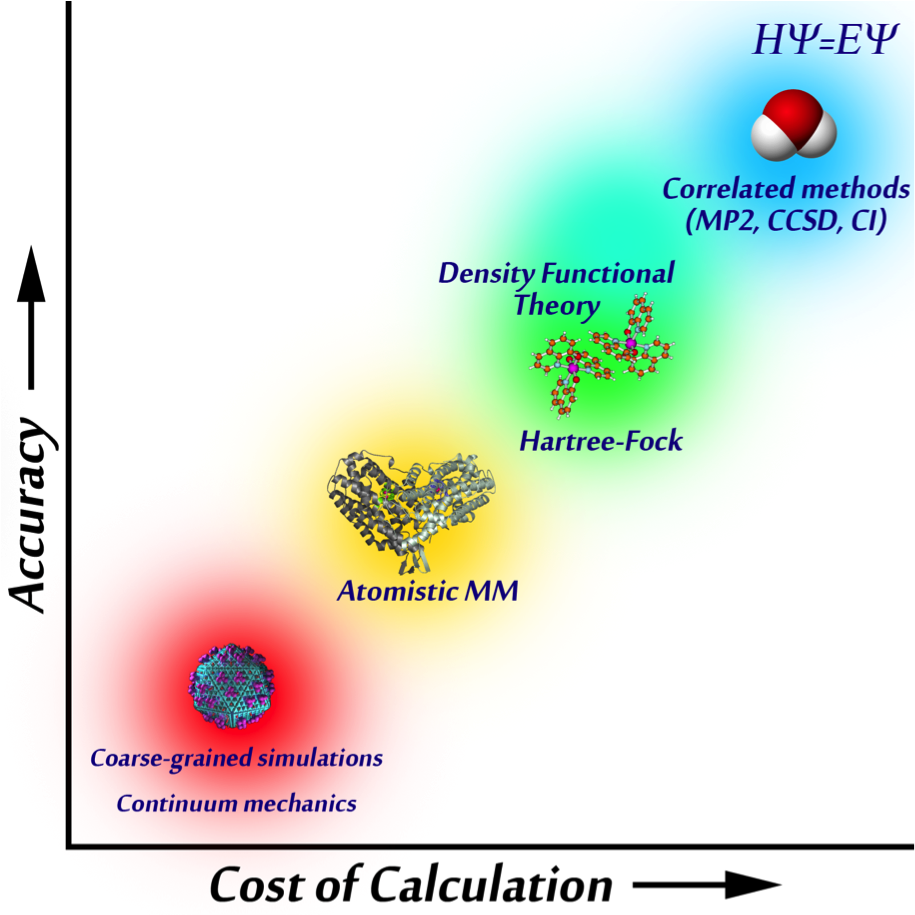
\includegraphics[width=10cm]{ladder.png}
\doxyfigcaption{An arrangement of simulation methods by accuracy vs. computational cost.}
\end{DoxyImage}


The main audience of Force\+Balance is the scientific community that uses and develops classical force fields. These force fields do not use the Schrodinger\textquotesingle{}s equation as a starting point; instead, the potential is entirely specified using elementary mathematical functions. Thus, the rigorous physical foundation is sacrificed but the computational cost is reduced by a factor of millions, enabling atomic-\/resolution simulations of large biomolecules on long timescales and allowing the study of problems like protein folding.

In classical force fields, relatively few parameters may be determined directly from experiment -\/ for instance, a chemical bond may be described using a harmonic spring with the experimental bond length and vibrational frequency. More often there is no experimentally measurable counterpart to a parameter -\/ for example, electrostatic interactions are often described as Coulomb interactions between pairs of atomic point \char`\"{}partial charges\char`\"{}, but the fractional charge assigned to each atom has no rigorous experimental of theoretical definition. To complicate matters further, most molecular motions arise from a combination of interactions and are sensitive to many parameters at once -\/ for example, the dihedral interaction term is intended to govern torsional motion about a bond, but these motions are modulated by the flexibility of the nearby bond and angle interactions as well as the nonbonded interactions on either side.

 
\begin{DoxyImage}
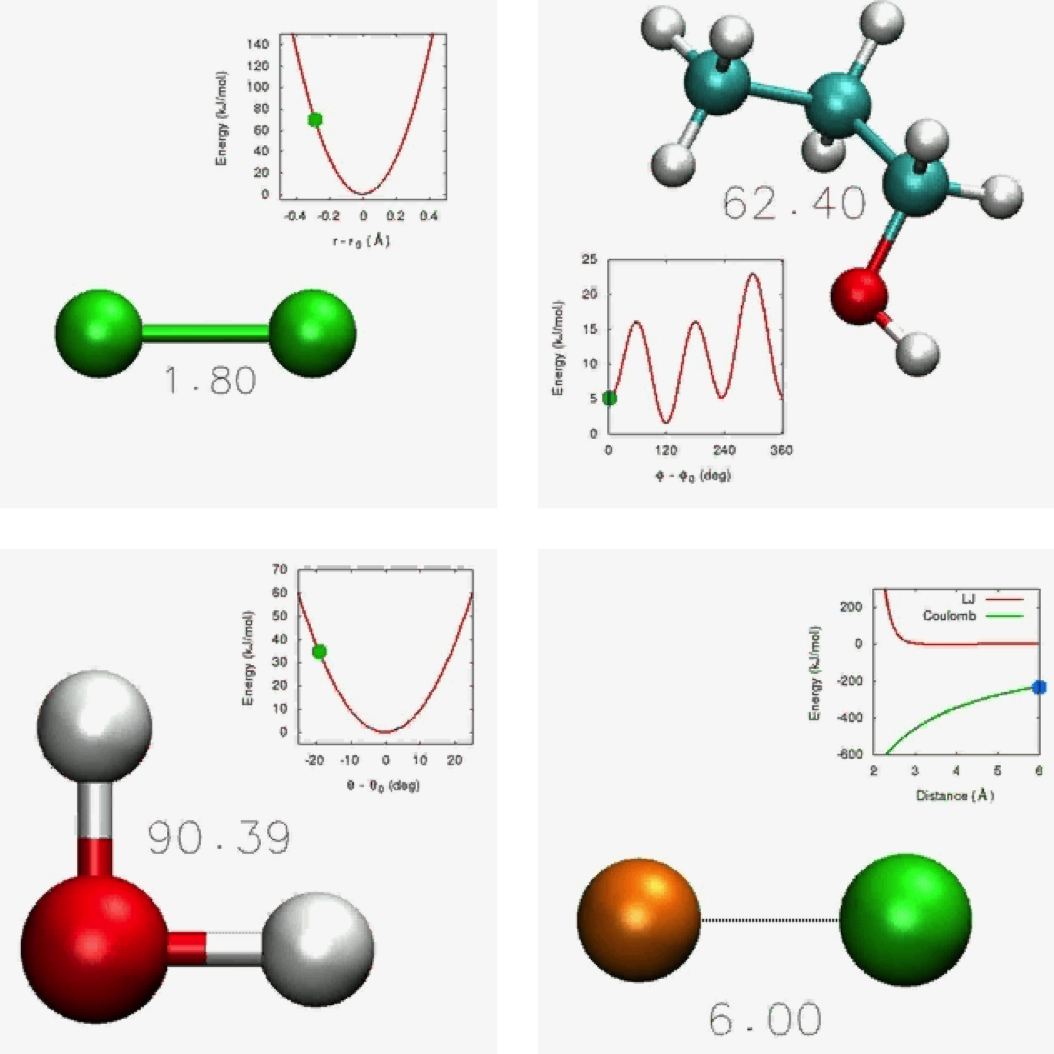
\includegraphics[width=10cm]{interactions.png}
\doxyfigcaption{An illustration of some interactions typically found in classical force fields.}
\end{DoxyImage}


For all of these reasons, force field parameterization is difficult. In the current practice, parameters are often determined by fitting to results from other calculations (for example, restrained electrostatic potential fitting (R\+E\+SP) for determining the partial charges) or chosen so that the simulation results match experimental measurements (for example, adjusting the partial charges on a solvent molecule to reproduce the bulk dielectric constant.) Published force fields have been modified by hand over decades to maximize their agreement with experimental observations (for example, adjusting some parameters in order to reproduce particular protein N\+MR structure) at the expense of reproducibility.\hypertarget{index_mission_statement}{}\subsubsection{Purpose and brief description of this program}\label{index_mission_statement}
Given this background, I can make the following statement. {\bfseries The purpose of Force\+Balance is to create force fields by applying a highly general and systematic process with explicitly specified input data and optimization methods, paving the way to higher accuracy and improved reproducibility. }

At a high level, Force\+Balance takes an empirical potential and a set of reference data as inputs, and tunes the parameters such that the simulations are able to reproduce the data as accurately as possible. Examples of reference data include energy and forces from high-\/level QM calculations, experimentally known molecular properties (e.\+g. polarizabilities and multipole moments), and experimentally measured bulk properties (e.\+g. density and dielectric constant).

Force\+Balance presents the problem of potential optimization in a unified and easily extensible framework. Since there are many empirical potentials in theoretical chemistry and similarly many types of reference data, significant effort is taken to provide an infrastructure which allows a researcher to fit any type of potential to any type of reference data.

Conceptually, a set of reference data (usually a physical quantity of some kind), in combination with a method for computing the corresponding quantity with the force field, is called a {\bfseries target}. For example\+:


\begin{DoxyItemize}
\item A force field can predict the density of a liquid by running N\+PT molecular dynamics, and this computed value can be compared against the experimental density.
\item A force field can be used to evaluate the energies and forces at several molecular geometries, and these can be compared against energies and forces from higher-\/level quantum chemistry calculations using these same geometries. This is known as {\bfseries force and energy matching}.
\item A force field can predict the multipole moments and polarizabilities of a molecule isolated in vacuum, and these can be compared against experimental measurements.
\end{DoxyItemize}

Within a target, the accuracy of the force field can be optimized by tuning the parameters to minimize the difference between the computed and reference quantities. One or more targets can be combined to produce an aggregate {\bfseries objective function} whose domain is the {\bfseries parameter space}. This objective function, which typically depends on the parameters in a complex way, is minimized using nonlinear optimization algorithms. The result is a force field which minimizes the errors for all of the targets.

 
\begin{DoxyImage}
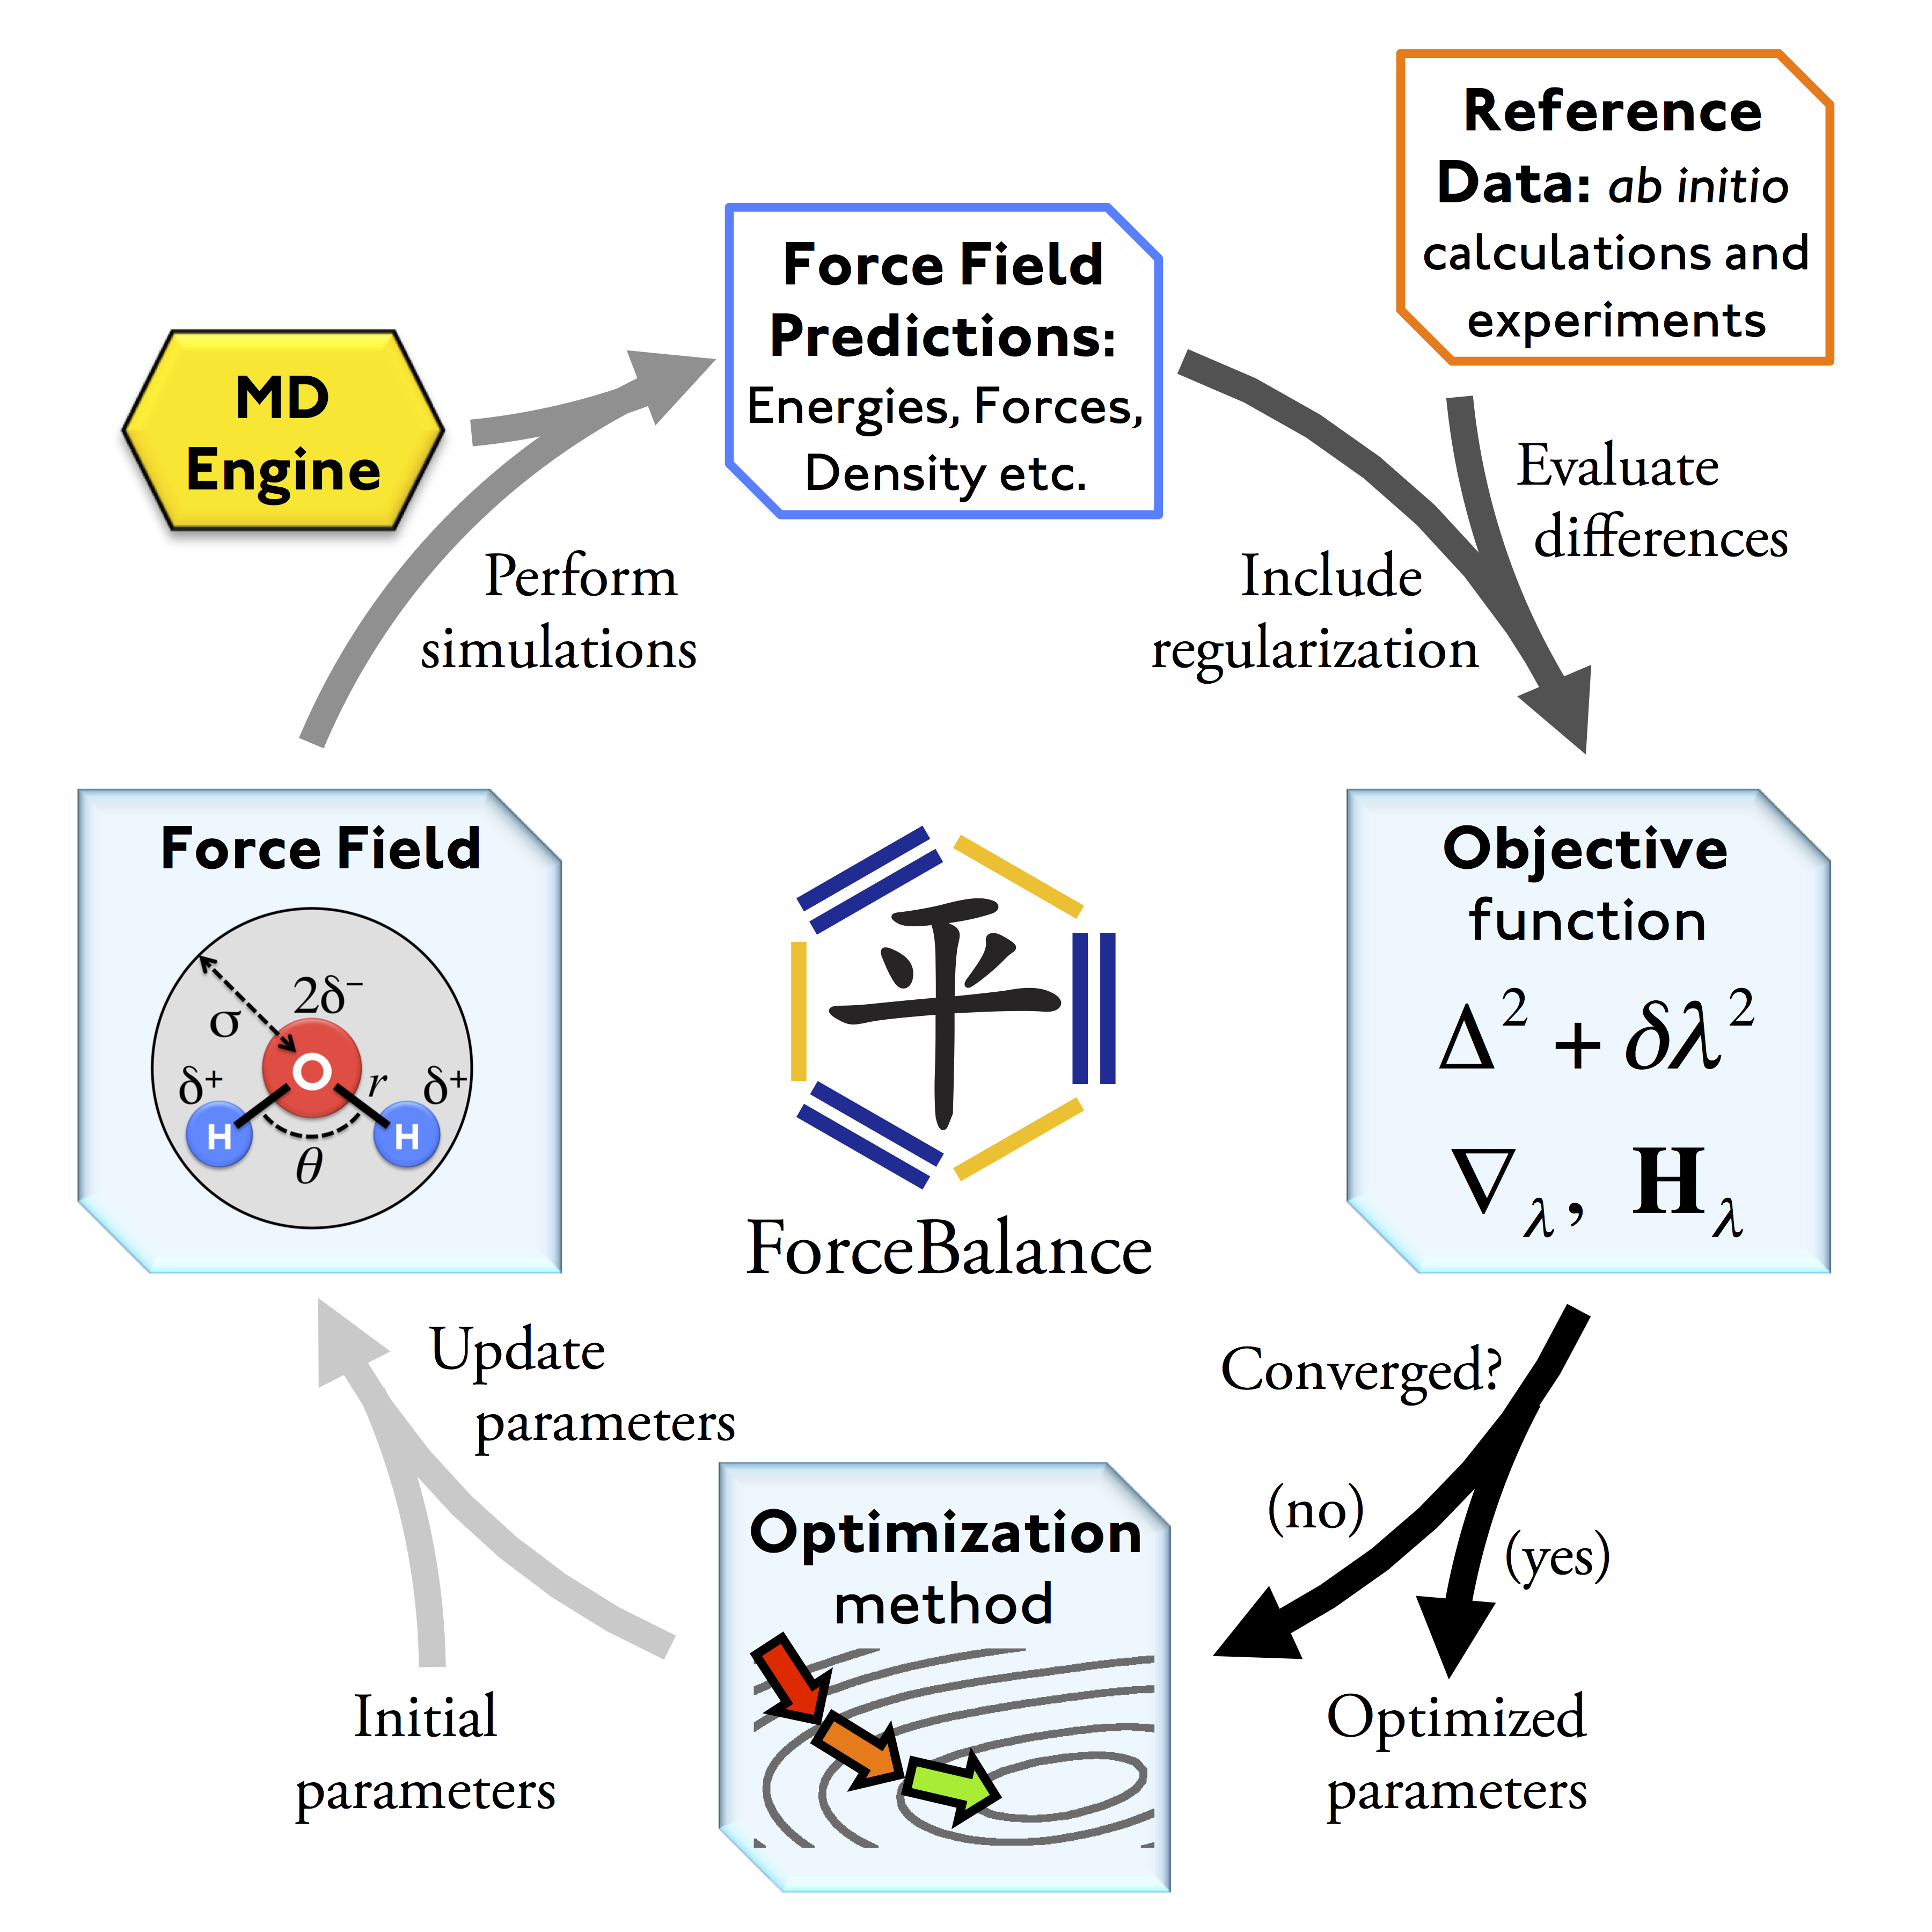
\includegraphics[height=10cm]{cycle.png}
\doxyfigcaption{The division of the potential optimization problem into three parts; the force field, targets and optimization algorithm.}
\end{DoxyImage}


The problem is now split into three main components; the force field, the targets, and the optimization algorithm. Force\+Balance uses this conceptual division to define three classes with minimal interdependence. Thus, if a researcher wishes to explore a new functional form, incorporate a new type of reference data or try a new optimization algorithm, he or she would only need to contribute to one branch of the program without having to restructure the entire code base.

The scientific problems and concepts that this program is based upon are further described in my Powerpoint presentations and publications, which can be found on the \href{https://simtk.org/home/forcebalance/}{\tt Sim\+TK website}.\hypertarget{index_credits}{}\subsection{Credits}\label{index_credits}

\begin{DoxyItemize}
\item Lee-\/\+Ping Wang is the principal developer and author. (2006-\/2019)
\item Yudong Qiu contributed the surface tension target, pure finite-\/difference for thermodynamic property gradients, the optimized geometry target, the Open\+MM implementation of the vibrational frequency target, the interface to Property\+Estimator, and other improvements when Force\+Balance is used with the S\+M\+I\+R\+N\+O\+FF force field. (2016-\/2019)
\item Jeffrey Wagner contributed modernized testing infrastructure and continuous integration, and assisted with developing the interface to the Open Force Field toolkit. (2019)
\item Hyesu Jang contributed modernized testing infrastructure with Jeff Wagner. (2019)
\item Simon Boothroyd contributed the interface to Property\+Estimator with Yudong Qiu. (2019)
\item Arthur Vigil contributed the unit testing framework and many unit tests, significant improvements to the automatic documentation generation, logging of output, graphical user interface, and various code improvements. (2012-\/2013)
\item Keri Mc\+Kiernan contributed the lipid bilayer target, starting from multiple initial conditions at each thermodynamic phase point, and several other features. (2012-\/2015)
\item Erik Brandt contributed the general thermodynamic property \char`\"{}\+Thermo\char`\"{} target. (2014)
\item Johnny Israeli contributed the Xml\+Script functionality that allows adjustable parameters to be read from embedded scripts in Open\+MM X\+ML files. (2012)
\item Matt Welborn contributed the parallelization-\/over-\/snapshots functionality in the general force matching module (2011, only in the older For\+Tune code).
\item Jiahao Chen contributed the call graph generator, the Q\+T\+P\+IE fluctuating-\/charge force field (which Lee-\/\+Ping implemented into G\+R\+O\+M\+A\+CS), the interface to the M\+O\+P\+AC semiempirical code, and many helpful discussions in 2009-\/2011. (Many of these are only in the older For\+Tune code)
\item Troy Van Voorhis provided scientific guidance and many of the central ideas as well as financial support during the time Lee-\/\+Ping was a graduate student (2006-\/2011).
\item Vijay Pande provided scientific guidance and financial support, and through the Sim\+Bios program gave this software a home on the Web at the \href{https://simtk.org/home/forcebalance/}{\tt Sim\+TK website}.
\item Todd Martinez provided scientific guidance and financial support.
\end{DoxyItemize}\hypertarget{index_funding}{}\subsection{Funding}\label{index_funding}
The development of this code has been supported in part by the following grants and awards\+:

N\+IH Grant R01 A\+I130684-\/02 A\+C\+S-\/\+P\+RF 58158-\/\+D\+N\+I6 N\+IH Grant U54 G\+M072970 Open Force Field Consortium 
\section{Installation}
\label{installation}
\Hypertarget{installation}
This section covers how to install Force\+Balance.

Currently only Linux is supported, though installation on other Unix-\/based systems (e.\+g. Mac OS) should also be straightforward.

Importantly, note that {\itshape Force\+Balance does not contain a simulation engine}. Instead it interfaces with simulation software like G\+R\+O\+M\+A\+CS, T\+I\+N\+K\+ER, A\+M\+B\+ER or Open\+MM; reference data is obtained from experimental measurements (consult the literature) or from quantum chemistry software (for example, N\+W\+Chem or Q-\/\+Chem).

Several interfaces to existing software packages are provided. However, if you use Force\+Balance for a research project, you should be prepared to write some simple Python code to interface with a software package of your choice. If you choose to do so, please contact me as I would be happy to include your contribution in the main distribution.\hypertarget{installation_installing_forcebalance}{}\subsection{Installing Force\+Balance using conda package manager}\label{installation_installing_forcebalance}
As of version 1.\+7.\+4, Force\+Balance is available as a package on the conda-\/forge channel. To install the package, make sure you are using an Anaconda/\+Miniconda Python distribution for Python versions 2.\+7, 3.\+5, 3.\+6, or 3.\+7, then run\+:

\begin{DoxyVerb}python setup.py install \end{DoxyVerb}


This will install Force\+Balance and all of the required dependencies. It will not install optional dependencies such as Open\+MM, Gromacs, A\+M\+B\+ER, Tinker, C\+C\+Tools/\+Work Queue, or the Open Force Field toolkit.\hypertarget{installation_installing_forcebalance}{}\subsection{Installing Force\+Balance using conda package manager}\label{installation_installing_forcebalance}
Force\+Balance is packaged as a Python module. Here are the installation instructions.

A quick preface\+: Installing software can be a real pain. I tried to make Force\+Balance easy to install by providing clear instructions and minimizing the number of dependencies; however, complications and challenges during installation happen all the time. If you are running into installation problems or having trouble resolving a dependency, please contact me.\hypertarget{installation_installing_forcebalance_prereq}{}\subsubsection{Prerequisites}\label{installation_installing_forcebalance_prereq}
Force\+Balance requires the following software packages\+:

\begin{DoxyItemize}
\item \href{http://www.python.org/}{\tt Python} version 2.\+7 \item \href{http://numpy.scipy.org/}{\tt Num\+Py} version 1.\+5 \item \href{http://www.scipy.org/}{\tt Sci\+Py} version 0.\+9\end{DoxyItemize}
The following packages are required for certain functionality\+:

\begin{DoxyItemize}
\item \href{http://lxml.de/}{\tt lxml} version 2.\+3.\+4 -\/ Python interface to libxml2 for parsing Open\+MM force field files \item \href{http://nd.edu/~ccl/software/}{\tt cctools} version 3.\+4.\+1 -\/ Cooperative Computing Tools from Notre Dame for distributed computing \item \href{https://matplotlib.org}{\tt matplotlib} version 2.\+0.\+2 -\/ Python plotting library which produces publication quality figures\end{DoxyItemize}
The following packages are used for documentation\+:

\begin{DoxyItemize}
\item \href{http://www.stack.nl/~dimitri/doxygen/}{\tt Doxygen} version 1.\+7.\+6.\+1 \item \href{http://code.foosel.org/doxypy}{\tt Doxypy} plugin for Doxygen \item La\+TeX software such as \href{http://www.tug.org/texlive/}{\tt Te\+X\+Live} \item The dot program from \href{http://www.graphviz.org/}{\tt graphviz} software package\end{DoxyItemize}
\hypertarget{installation_installing_forcebalance_install}{}\subsubsection{Installing}\label{installation_installing_forcebalance_install}
To install the package, first extract the tarball that you downloaded from the webpage using the command\+:

\begin{DoxyVerb}tar xvzf ForceBalance-[version].tar.gz \end{DoxyVerb}


Alternatively, download the newest Subversion revision from the Sim\+TK website\+:

\begin{DoxyVerb}svn checkout https://simtk.org/svn/forcebalance \end{DoxyVerb}


Upon extracting the distribution you will see this directory structure\+:

\begin{DoxyVerb} <root>
   +- bin
   |   |- <Executable scripts>
   +- src
   |   |- <ForceBalance source files>
   +- ext
   |   |- <Extensions; self-contained software packages that are used by ForceBalance>
   +- studies
   |   +- <ForceBalance example jobs>
   +- doc
   |   +- callgraph
   |   |   |- <Stuff for making a call graph>
   |   +- Images
   |   |   |- <Images for the website and PDF manual>
   |   |- make-all-documentation.sh (Create the documentation)
   |   |- <Below are documentation chapters in Doxygen format>
   |   |- introduction.txt
   |   |- installation.txt
   |   |- usage.txt
   |   |- tutorial.txt
   |   |- glossary.txt
   |   |- <The above files are concatenated into mainpage.py>
   |   |- make-all-documentation.sh (Command for making all documentation)
   |   |- make-option-index.py (Create the option index documentation chapter)
   |   |- header.tex (Customize the LaTex documentation)
   |   |- add-tabs.py (Adds more navigation tabs to the webpage)
   |   |- DoxygenLayout.xml (Removes a navigation tab from the webpage)
   |   |- doxygen.cfg (Main configuration file for Doxygen)
   |   |- ForceBalance-Manual.pdf (PDF manual, but the one on the SimTK website is probably newer)
   |- PKG-INFO (Auto-generated package information)
   |- README.txt (Points to the SimTK website)
   |- setup.py (Python script for installation) \end{DoxyVerb}


To install the code into your default Python location, run this (you might need to be root)\+:

\begin{DoxyVerb}python setup.py install \end{DoxyVerb}


You might not have root permissions, or you may want to install the package somewhere other than the default location. You can install to a custom location (for example, to /home/leeping/local) by running\+:

\begin{DoxyVerb}python setup.py install --prefix=/home/leeping/local \end{DoxyVerb}


Assuming your Python version is 2.\+7, the executable scripts will be placed into {\ttfamily /home/leeping/local/bin} and the module will be placed into {\ttfamily /home/leeping/local/lib/python2.7/site-\/packages/forcebalance}.

Note that Python does not always recognize installed modules in custom locations. Any one of the three below options will work for adding custom locations to the Python search path for installed modules\+:

\begin{DoxyVerb}ln -s /home/leeping/local /home/leeping/.local \end{DoxyVerb}
 \begin{DoxyVerb}export PYTHONUSERBASE=/home/leeping/local \end{DoxyVerb}
 \begin{DoxyVerb}export PYTHONPATH=$PYTHONPATH:/home/leeping/local/lib/python2.7 \end{DoxyVerb}


As with the installation of any software, there are potential issues with dependencies (for example, scipy and lxml.) One way to resolve dependencies is to use the Enthought Python Distribution (E\+PD), which contains all of the required packages and is free for academic users. Install E\+PD from the \href{http://www.enthought.com/products/epd.php}{\tt Enthought website}. Configure your environment by running both of the commands below (assuming Enthought was installed to {\ttfamily  /home/leeping/opt/epd-\/7.3.\+2 }, with the python executable in the {\ttfamily bin} subdirectory)\+:

\begin{DoxyVerb} export PATH=/home/leeping/opt/epd-7.3.2/bin:$PATH
 export PYTHONUSERBASE=/home/leeping/opt/epd-7.3.2 \end{DoxyVerb}


An alternative option is to use Anaconda2, that can be downloaded \href{https://www.continuum.io/downloads}{\tt the Continuum website}. It is also free for academic users.

\begin{DoxyVerb} export PATH=/home/leeping/opt/anaconda2/bin:$PATH \end{DoxyVerb}


Once you have done this, the Numpy, Scipy, Matplotlib and lxml dependency issues should be resolved and Force\+Balance will run without any problems.

Here are a list of installation notes (not required if you install Force\+Balance into the Enthought Python Distribution). These notes assume that Python and other packages are installed into \$\+H\+O\+ME/local.

\begin{DoxyItemize}
\item The installation of Numpy, Scipy and lxml may be facilitated by installing the {\ttfamily pip} package -\/ simply run a command like {\ttfamily pip install numpy}. \item Scipy requires a B\+L\+AS (Basic Linear Algebra Subroutines) library to be installed. On certain Linux distributions such as Ubuntu, the B\+L\+AS libraries and headers can be found on the repository (run {\ttfamily sudo apt-\/get install libblas-\/dev}). Also, B\+L\+AS is provided by libraries such as A\+T\+L\+AS (Automatically Tuned Linear Algebra Software) or the Intel M\+KL (Math Kernel Library) for Intel processors. To compile Scipy with Intel\textquotesingle{}s M\+KL, follow the guide on \href{http://software.intel.com/en-us/articles/numpy-scipy-with-mkl}{\tt Intel\textquotesingle{}s website}. To use A\+T\+L\+AS, install the package from the \href{http://math-atlas.sourceforge.net}{\tt A\+T\+L\+AS website } and set the A\+T\+L\+AS environment variable (for example, {\ttfamily export A\+T\+L\+AS=\$\+H\+O\+ME/local/lib/libatlas.so}) before installing Scipy. \item {\ttfamily lxml} is a Python interface to the libxml2 X\+ML parser. After much ado, I decided to use {\ttfamily lxml} instead of the {\ttfamily xml} module in Python\textquotesingle{}s standard library for several reasons ({\ttfamily xml} contains only limited support for X\+Path, scrambles the ordering of attributes in an element, etc.) The downside is that it can be harder to install. Installation instructions can be found on the \href{http://lxml.de/installation.html}{\tt lxml website} but summarized here. The packages {\ttfamily libxml2} and {\ttfamily libxslt} need to be installed first, and in that order. On Ubuntu, run {\ttfamily sudo apt-\/get install libxml2-\/dev libxslt1-\/dev}. To compile from source, run {\ttfamily ./configure --prefix=\$\+H\+O\+ME/local --with-\/python=\$\+H\+O\+ME/local}. Then run {\ttfamily make} followed by {\ttfamily make install}. Python itself needs to be compiled with {\ttfamily --enable-\/shared} for this to work. Finally, download and unzip {\ttfamily lxml}, then run {\ttfamily  python setup.\+py install --prefix=\$\+H\+O\+ME/local }.\end{DoxyItemize}
\hypertarget{installation_create_doc}{}\subsection{Create documentation}\label{installation_create_doc}
This documentation is created by Doxygen with the Doxypy plugin. To create new documentation or expand on what\textquotesingle{}s here, follow the examples in the source code or visit the Doxygen home page.

To create this documentation from the source files, go to the {\ttfamily doc} directory in the distribution and run {\ttfamily  doxygen doxygen.\+cfg } to generate the H\+T\+ML documentation and La\+TeX source files. Run the {\ttfamily add-\/tabs.\+py} script to generate the extra navigation tabs for the H\+T\+ML documentation. Then go to the {\ttfamily latex} directory and type in {\ttfamily make} to build the P\+DF manual (You will need a La\+TeX distribution for this.) All of this is automated by running {\ttfamily make-\/all-\/documentation.\+sh}.\hypertarget{installation_install_gmxx2}{}\subsection{Installing G\+R\+O\+M\+A\+C\+S-\/\+X2}\label{installation_install_gmxx2}
{\itshape  G\+R\+O\+M\+A\+C\+S-\/\+X2 is not required for Force\+Balance and is currently deprecated. Installation is not recommended. This section is retained for your information and in case I choose to revive the software. }

I have provided a specialized version of G\+R\+O\+M\+A\+CS (dubbed version 4.\+0.\+7-\/\+X2) on the \href{https://simtk.org/home/forcebalance/}{\tt Sim\+TK website} which interfaces with Force\+Balance through the abinitio\+\_\+gmxx2 module. Although interfacing with unmodified simulation software is straightforward, G\+R\+O\+M\+A\+C\+S-\/\+X2 is optimized for force field optimization and makes things much faster.

G\+R\+O\+M\+A\+C\+S-\/\+X2 contains major modifications from G\+R\+O\+M\+A\+CS 4.\+0.\+7. Most importantly, it enables computation of the objective function and its analytic derivatives for rapid energy and force matching. There is also an implementation of the Q\+T\+P\+IE fluctuating-\/charge polarizable force field, and the beginnings of a G\+R\+O\+M\+A\+C\+S/\+Q-\/\+Chem interface (carefully implemented but not extensively tested). Most of the changes were added in several new source files (less than ten)\+: {\ttfamily qtpie.\+c}, {\ttfamily fortune.\+c}, {\ttfamily fortune\+\_\+utils.\+c}, {\ttfamily fortune\+\_\+vsite.\+c}, {\ttfamily fortune\+\_\+nb\+\_\+utils.\+c}, {\ttfamily zmatrix.\+c} and their corresponding header files, and {\ttfamily fortunerec.\+h} for the force matching data structure. The name \textquotesingle{}fortune\textquotesingle{} derives from back when this code was called For\+Tune.

The force matching functions are turned on by calling {\ttfamily mdrun} with the command line argument {\ttfamily \textquotesingle{}-\/fortune\textquotesingle{}} ; without this option, there should be no impact on the performance of normal MD simulations.

Force\+Balance interfaces with G\+R\+O\+M\+A\+C\+S-\/\+X2 through the functions in {\ttfamily abinitio\+\_\+gmxx2.\+py} ; the objective function and derivatives are computed and printed to output files. The interface is defined in {\ttfamily fortune.\+c} on the G\+R\+O\+M\+A\+CS side. Force\+Balance needs to know where the G\+R\+O\+M\+A\+C\+S-\/\+X2 executables are located, and this is specified using the {\ttfamily gmxpath} option in the input file.\hypertarget{installation_install_gmxx2_prerequisites}{}\subsubsection{Prerequisites for G\+R\+O\+M\+A\+C\+S-\/\+X2}\label{installation_install_gmxx2_prerequisites}
G\+R\+O\+M\+A\+C\+S-\/\+X2 needs the base G\+R\+O\+M\+A\+CS requirements and several other libraries.

\begin{DoxyItemize}
\item F\+F\+TW version 3.\+3 \item G\+Lib version 2.\+0 \item Intel M\+KL library\end{DoxyItemize}
G\+Lib is the utility library provided by the G\+N\+O\+ME foundation (the folks who make the G\+N\+O\+ME desktop manager and G\+T\+K+ libraries). G\+R\+O\+M\+A\+C\+S-\/\+X2 requires G\+Lib for its hash table (dictionary).

G\+Lib and F\+F\+TW can be compiled from source, but it is much easier if you\textquotesingle{}re using a Linux distribution with a package manager. If you\textquotesingle{}re running Ubuntu or Debian, run {\ttfamily sudo apt-\/get install libglib2.\+0-\/dev libfftw3-\/dev}; if you\textquotesingle{}re using Cent\+OS or some other distro with the yum package manager, run {\ttfamily sudo yum install glib2-\/devel.\+x86\+\_\+64 fftw3-\/devel.\+x86\+\_\+64} (or replace {\ttfamily x86\+\_\+64} with {\ttfamily i386} if you\textquotesingle{}re not on a 64-\/bit system.

G\+R\+O\+M\+A\+C\+S-\/\+X2 requires the Intel Math Kernel Library (M\+KL) for linear algebra. In principle this requirement can be lifted if I rewrite the source code, but it\textquotesingle{}s a lot of trouble, plus M\+KL is faster than other implementations of B\+L\+AS and L\+A\+P\+A\+CK.

The Intel M\+KL can be obtained from the Intel website, free of charge for noncommercial use. Currently G\+R\+O\+M\+A\+C\+S-\/\+X2 is built with M\+KL version 10.\+2, which ships with compiler version 11.\+1/072 ; this is not the newest version, but it can still be obtained from the Intel website after you register for a free account.

After installing these packages, extract the tarball that you downloaded from the website using the command\+:

\begin{DoxyVerb}tar xvjf gromacs-[version]-x2.tar.bz2 \end{DoxyVerb}


The directory structure is identical to G\+R\+O\+M\+A\+CS 4.\+0.\+7, but I added some shell scripts. {\ttfamily Build.\+sh} will run the configure script using some special options, compile the objects, create the executables and install them; you will probably need to modify it slightly for your environment. The comments in the script will help further with installation.

Don\textquotesingle{}t forget to specify the install location of the G\+R\+O\+M\+A\+C\+S-\/\+X2 executables in the Force\+Balance input file! 
\section{Usage}
\label{usage}
\Hypertarget{usage}
This page describes how to use the Force\+Balance software.

A good starting point for using this software package is to run the scripts contained in the {\ttfamily bin} directory on the example jobs in the {\ttfamily studies} directory.

{\ttfamily Force\+Balance.\+py} is the main executable script for force field optimization. It requires an input file and a \hyperlink{usage_directory_structure}{Directory structure}. {\ttfamily Make\+Input\+File.\+py} will create an example input file containing all options, their default values, and a short description for each option.\hypertarget{usage_input_file}{}\subsection{Input file}\label{usage_input_file}
A minimal input file for Force\+Balance might look something like this\+:

\begin{DoxyVerb} $options
 jobtype newton
 forcefield water.itp
 $end
 
 $target
 name cluster-02
 type abinitio_gmx
 $end
 
 $target
 name cluster-03
 type abinitio_gmx
 $end\end{DoxyVerb}


Global options for a Force\+Balance job are given in the {\ttfamily \$options} section while the settings for each Target are given in the {\ttfamily \$target} sections. These are the only two section types.

The most important general options to note are\+: {\ttfamily jobtype} specifies the optimization algorithm to use and {\ttfamily forcefield} specifies the force field file name (there may be more than one of these). The most important target options to note are\+: {\ttfamily name} specifies the target name and {\ttfamily type} specifies the type of target (must correspond to a subdirectory in {\ttfamily targets/} ). All options are explained in the Option Index.\hypertarget{usage_directory_structure}{}\subsection{Directory structure}\label{usage_directory_structure}
The directory structure for our example job would look like\+:

\begin{DoxyVerb} <root>
   +- forcefield
   |   |- water.itp
   +- targets
   |   +- cluster-02
   |   |   +- settings (contains job settings)
   |   |   |   |- shot.mdp
   |   |   |   |- topol.top
   |   |   |- all.gro (contains geometries)
   |   |   |- qdata.txt (contains QM data)
   |   +- cluster-03
   |   |   +- settings
   |   |   |   |- shot.mdp
   |   |   |   |- topol.top
   |   |   |- all.gro
   |   |   |- qdata.txt
   |   +- <more target directories>
   |- input.in
   +- temp
   |   |- iter_0001
   |   |- iter_0002
   |   |   |- <files generated during runtime>
   +- result
   |   |- water.itp (Optimized force field, generated on completion)
   |- input.in (ForceBalance input file)\end{DoxyVerb}


The top-\/level directory names {\bfseries forcefield} and {\bfseries targets} are fixed and cannot be changed. {\bfseries forcefield} contains the force field files that you\textquotesingle{}re optimizing, and {\bfseries targets} contains all of the reference data as well as the input files for simulating that data using the force field. Each subdirectory in {\bfseries targets} corresponds to a single target, and its contents depend on the specific kind of target and its corresponding {\ttfamily Target} class.

The {\bfseries temp} directory is the temporary workspace of the program, and the {\bfseries result} directory is where the optimized force field files are deposited after the optimization job is done. These two directories are created if not already there.

Note the force field file, {\ttfamily water.\+itp} and the two fitting targets {\ttfamily cluster-\/02} and {\ttfamily cluster-\/03} match the {\ttfamily target} sections in the input file. There are two energy and force matching targets here; each directory contains the relevant geometries (in {\ttfamily all.\+gro} ) and reference data (in {\ttfamily qdata.\+txt} ).\hypertarget{usage_targets}{}\subsection{Setting up the targets}\label{usage_targets}
There are many targets one can choose from.

\begin{DoxyItemize}
\item Energy and force matching -\/ this is the oldest functionality and the most robust. Enabled in G\+R\+O\+M\+A\+CS, Open\+MM, T\+I\+N\+K\+ER, A\+M\+B\+ER. \item Electrostatic potential fitting via the R\+E\+SP method. Enabled in G\+R\+O\+M\+A\+CS and A\+M\+B\+ER. \item High-\/performance interaction energies -\/ intended for the same two fragments in many conformations. Enabled in G\+R\+O\+M\+A\+CS. \item General binding energies -\/ intended for highly diverse collections of complexes and fragments. Enabled in T\+I\+N\+K\+ER. \item Normal mode frequencies. Enabled in T\+I\+N\+K\+ER. \item Condensed-\/phase properties; currently enabled only for density and enthalpy of vaporization of water. Enabled in Open\+MM. \item Basis set coefficient fitting; enabled in psi4 (experimental)\end{DoxyItemize}
One feature of Force\+Balance is that targets can be linearly combined to produce an aggregate objective function. For example, our recently developed polarizable water model contains energy and force matching, binding energies, normal mode frequencies, density, and enthalpy of vaporization. With the A\+M\+O\+E\+BA functional form and 19 adjustable parameters, we developed a highly accurate model that fitted all of these properties to very high accuracy.

Due to the diverse nature of these calculations, they need to be set up in a specific way that is recognized by Force\+Balance. The setup is different for each type of simulation, and we invite you to learn by example through looking at the files in the {\ttfamily studies} directory.\hypertarget{usage_energy_force_matching}{}\subsubsection{Energy and force matching}\label{usage_energy_force_matching}
In these relatively simple simulations, the objective function is computed from the squared difference in the potential energy and forces (gradients) between the force field and reference (QM) method, evaluated at a number of stored geometries called {\itshape snapshots}. The mathematics are implemented in {\ttfamily abinitio.\+py} while the interfaces to simulation software exist in derived classes in {\ttfamily gmxio.\+py}, {\ttfamily tinkerio.\+py}, {\ttfamily amberio.\+py} and {\ttfamily openmmio.\+py}.

All energy and force matching targets require a {\itshape coordinate trajectory file} ({\ttfamily all.\+gro} ) and a {\itshape  quantum data file } ({\ttfamily qdata.\+txt} ). The coordinate trajectory file contains the Cartesian coordinates of the snapshots, preferably in the file format of the simulation software used ({\ttfamily all.\+gro} is the most extensively tested.) The quantum data file is formatted according to a very simple specification\+:

\begin{DoxyVerb} JOB 0
 COORDS x1 y1 z1 x2 y2 z2 ... (floating point numbers in Angstrom)
 ENERGY (floating point number in Hartree)
 FORCES fx1 fy1 fz1 ... (floating point numbers in Hartree/bohr - this is a misnomer because they are actually gradients, which differ by a sign from the forces.)
 
 JOB 1
 ...\end{DoxyVerb}


The coordinates in the quantum data file should be consistent with the coordinate trajectory file, although Force\+Balance will use the latter most of the time. It is easy to generate the quantum data file from parsing the output of quantum chemistry software. Force\+Balance contains methods for parsing Q-\/\+Chem output files in the {\ttfamily molecule.\+py} class.

In addition to {\ttfamily all.\+gro} and {\ttfamily qdata.\+txt} , the simulation setup files are required. These contain settings needed by the simulation software for the calculation to run. For Gromacs calculations, a topology (.top) file and a run parameter file (.mdp) are required. These should be placed in the {\ttfamily settings} subdirectory within the directory belonging to the target.

As a side note\+: If you wish to tune a number in the .mdp file, simply move it to the {\ttfamily forcefield} directory and specify it as a force field file. Force\+Balance will now be able to tune any highlighted parameters in the file, although it will also place copies of this file in all target directories within {\ttfamily temp} while the program is running.\hypertarget{usage_Electrostatic}{}\subsubsection{potentials}\label{usage_Electrostatic}
Force\+Balance contains methods for evaluating electrostatic potentials given a collection of point charges. At this time, this functionality is very experimental and risky to use for systems containing more than one molecule. This is because Force\+Balance evaluates the electrostatic potentials internally, and we don\textquotesingle{}t have an infrastructure for building a full topology consisting of many molecules. Currently, we assume that the electrostatic potential fitting contains only one molecule.

Once again, the coordinate trajectory file and quantum data files are used to specify the calculation. However, now the coordinates for evaluating the potential, and the reference potential values, are included\+:

\begin{DoxyVerb} JOB 0
 COORDS x1 y1 z1 x2 y2 z2 ...
 ENERGY e
 FORCES fx1 fy1 fz1 ...
 ESPXYZ ex1 ey1 ez1 ex2 ey2 ez2 ... 
 ESPVAL ev1 ev2 ev3 ..\end{DoxyVerb}
\hypertarget{usage_running_software}{}\subsection{Running the optimization}\label{usage_running_software}
To run Force\+Balance, make sure the calculation is set up properly (refer to the above sections), and then type in\+:

{\bfseries  Force\+Balance.\+py input.\+in }

In general it\textquotesingle{}s impossible to set up a calculation perfectly the first time, in which case the calculation will crash. Force\+Balance will try to print helpful error messages to guide you toward setting up your calculation properly.

Further example inputs and outputs are given in the Tutorial section. 
\section{Tutorial}
\label{tutorial}
\Hypertarget{tutorial}
This is a tutorial page, but if you haven\textquotesingle{}t installed Force\+Balance yet please go to the Installation page first.

It is very much in process, and there are many more examples to come.\hypertarget{tutorial_tip4p}{}\subsection{Fitting a T\+I\+P4\+P potential to Q\+M cluster calculations}\label{tutorial_tip4p}
After everything is installed, go to the {\ttfamily studies/001\+\_\+water\+\_\+tutorial} directory in the distribution. Extract the {\ttfamily targets.\+tar.\+bz2} archive file. Now execute\+:

\begin{DoxyVerb} ForceBalance.py very_simple.in\end{DoxyVerb}


If the installation was successful, you will get an output file similar to {\ttfamily very\+\_\+simple.\+out} . What follows is a description of the output file and what Force\+Balance is actually doing.

Force\+Balance begins by reading the force field files from the {\ttfamily forcefield} directory. The parameters to be optimized are specified in the parameter file by adding a special comment inside the file. For example, in the {\ttfamily water.\+itp} file, we specify that the two van der Waals parameters on oxygen are to be optimized, using the following syntax\+:

\begin{DoxyVerb} OW     8     15.99940     0.000       A    3.15365e-01  6.48520e-01 ; PRM 5 6\end{DoxyVerb}


The comment {\ttfamily P\+RM 5 6} signals that \char`\"{}the parameters in fields 5
 and 6 are to be optimized.\char`\"{} The force field parser stores the physical value of the parameter and gives the parameter a name. These are printed out in the output file\+:

\begin{DoxyVerb} Reading force field from file: water.itp
 #=========================================================#
 #|  Starting parameter indices, physical values and IDs  |#
 #=========================================================#
    0 [  3.1537e-01 ] : VDWS:OW
    1 [  6.4852e-01 ] : VDWT:OW
    2 [  9.5720e-02 ] : BONDSB:HWOW
    3 [  5.0242e+05 ] : BONDSK:HWOW
    4 [  1.0452e+02 ] : ANGLESB:HWOWHW
    5 [  6.2802e+02 ] : ANGLESK:HWOWHW
    6 [  5.2000e-01 ] : COUL:SOL-2 COUL:SOL-3
    7 [ -1.0400e+00 ] : COUL:SOL-4
    8 [  1.2800e-01 ] : VSITE3B:SOL-4 VSITE3A:SOL-4
 -----------------------------------------------------------\end{DoxyVerb}


The next section it prints out are a set of rescaling factors which are important for various aspects of the optimization. They are discussed further in this \href{https://simtk.org/forums/viewtopic.php?f=710&t=3827}{\tt forum post}. For now it suffices to say that these values represent the natural size of the parameter, or more specifically how much the parameter is expected to vary.

\begin{DoxyVerb} #========================================================#
 #|     Rescaling Factors (Lower Takes Precedence):      |#
 #========================================================#
    BONDSB                               : 5.29177e-02
    BONDSK                               : 9.37583e+05
    VSITE3A                              : 5.29177e-02
    VSITE3B                              : 5.29177e-02
    ANGLESB                              : 5.72958e+01
    VDWS                                 : 5.29177e-02
    ANGLESK                              : 6.05928e+02
    COUL                                 : 1.00000e+00
    VDWT                                 : 2.47894e+00
 ----------------------------------------------------------\end{DoxyVerb}


Next, it prints out user-\/specified options that pertain to the force field the targets, the objective function and the optimizer. Options that are left at their default values (in this case, most) are not printed out. Use {\ttfamily verbose\+\_\+options True} in the input file to print out all of the options.

Now for the good stuff -\/ the optimizer begins. Force\+Balance computes each target and prints out an indicator for each one, then provides a breakdown of the overall objective function\+:

\begin{DoxyVerb} #========================================================#
 #|                    Main Optimizer                    |#
 #|        Newton-Raphson Mode (Adaptive Radius)         |#
 #========================================================#
 
 #=======================================================================#
 #|  Target: cluster-06 Type: AbInitio_GMX Objective = 1.12035e-01      |#
 #|                              Difference   Denominator     Percent   |#
 #|  Physical Variable           (Calc-Ref)     RMS (Ref)   Difference  |#
 #=======================================================================#
     Energy (kJ/mol)                 9.4124       27.3135     34.4605% 
     Gradient (kJ/mol/A)            39.1963      119.0841     32.9148% 
 -------------------------------------------------------------------------
 #=======================================================================#
 #|  Target: cluster-12 Type: AbInitio_GMX Objective = 1.04039e-01      |#
 #|                              Difference   Denominator     Percent   |#
 #|  Physical Variable           (Calc-Ref)     RMS (Ref)   Difference  |#
 #=======================================================================#
     Energy (kJ/mol)                15.2291       47.3455     32.1658% 
     Gradient (kJ/mol/A)            38.5401      118.0240     32.6545% 
 -------------------------------------------------------------------------
 #====================================================================#
 #|                   Objective Function Breakdown                   |#
 #|   Target Name              Residual  x  Weight  =  Contribution  |#
 #====================================================================#
 cluster-06                     0.11203      0.500      5.60173e-02 
 cluster-12                     0.10404      0.500      5.20195e-02 
 Regularization                 0.00000      1.000      0.00000e+00 
 Total                                                  1.08037e-01 
 ----------------------------------------------------------------------
   Step       |k|        |dk|       |grad|       -=X2=-     Delta(X2)    StepQual
      0   0.000e+00   0.000e+00   3.206e+00   1.08037e-01   0.000e+00      0.000\end{DoxyVerb}


In this example job, the targets were QM energies and forces for clusters of 6 and 12 water molecules. In the initial step (using the default T\+I\+P4P parameters) and for the first target (6-\/mers), the R\+MS error for energies is 9.\+4124 k\+J/mol (34\% of the variance in the QM energies themselves), and the R\+MS error for atomistic forces is 32\% (again, scaled to the variance of the QM forces). Similar information is printed out for the 12-\/mers. Each target contributes to the overall objective function, whose value is 1.\+080e-\/01. The parameters are at their initial values, which means that any penalty function will have a value of zero (the Regularization term).

Next, Force\+Balance takes a step in the parameter space. The default algorithm (a variation of Newton-\/\+Raphson) uses first and second derivative information; the gradient is printed to the screen, as is the parameter step.

\begin{DoxyVerb} #========================================================#
 #|                    Total Gradient                    |#
 #========================================================#
    0 [ -1.36605285e-01 ] : VDWS:OW
    1 [ -2.24335748e-01 ] : VDWT:OW
    2 [ -3.14688760e+00 ] : BONDSB:HWOW
    3 [  3.54975985e-01 ] : BONDSK:HWOW
    4 [ -3.24607484e-01 ] : ANGLESB:HWOWHW
    5 [  8.92900123e-02 ] : ANGLESK:HWOWHW
    6 [ -7.50893285e-02 ] : COUL:SOL-2 COUL:SOL-3
    7 [ -2.44318391e-01 ] : COUL:SOL-4
    8 [ -2.23561237e-02 ] : VSITE3B:SOL-4 VSITE3A:SOL-4
 ----------------------------------------------------------
 
 Levenberg-Marquardt: Newton-Raphson step found (length 1.000e-01),  0.92958359 added to Hessian diagonal
 #========================================================#
 #|   Mathematical Parameters (Current + Step = Next)    |#
 #========================================================#
    0 [  0.0000e+00 + 2.3057e-02 =  2.3057e-02 ] : VDWS:OW
    1 [  0.0000e+00 + 3.7320e-02 =  3.7320e-02 ] : VDWT:OW
    2 [  0.0000e+00 + 5.7207e-03 =  5.7207e-03 ] : BONDSB:HWOW
    3 [  0.0000e+00 - 3.8228e-02 = -3.8228e-02 ] : BONDSK:HWOW
    4 [  0.0000e+00 + 8.6160e-03 =  8.6160e-03 ] : ANGLESB:HWOWHW
    5 [  0.0000e+00 - 7.4597e-02 = -7.4597e-02 ] : ANGLESK:HWOWHW
    6 [  0.0000e+00 - 7.4155e-03 = -7.4155e-03 ] : COUL:SOL-2 COUL:SOL-3
    7 [  0.0000e+00 + 2.9107e-02 =  2.9107e-02 ] : COUL:SOL-4
    8 [  0.0000e+00 + 6.3479e-03 =  6.3479e-03 ] : VSITE3B:SOL-4 VSITE3A:SOL-4
 ----------------------------------------------------------
 #========================================================#
 #|     Physical Parameters (Current + Step = Next)      |#
 #========================================================#
    0 [  3.1537e-01 + 1.2201e-03 =  3.1659e-01 ] : VDWS:OW
    1 [  6.4852e-01 + 9.2513e-02 =  7.4103e-01 ] : VDWT:OW
    2 [  9.5720e-02 + 3.0273e-04 =  9.6023e-02 ] : BONDSB:HWOW
    3 [  5.0242e+05 - 3.5842e+04 =  4.6657e+05 ] : BONDSK:HWOW
    4 [  1.0452e+02 + 4.9366e-01 =  1.0501e+02 ] : ANGLESB:HWOWHW
    5 [  6.2802e+02 - 4.5200e+01 =  5.8282e+02 ] : ANGLESK:HWOWHW
    6 [  5.2000e-01 - 7.4155e-03 =  5.1258e-01 ] : COUL:SOL-2 COUL:SOL-3
    7 [ -1.0400e+00 + 2.9107e-02 = -1.0109e+00 ] : COUL:SOL-4
    8 [  1.2800e-01 + 3.3591e-04 =  1.2834e-01 ] : VSITE3B:SOL-4 VSITE3A:SOL-4
 ----------------------------------------------------------\end{DoxyVerb}


Note that the step length is limited to a \char`\"{}trust radius\char`\"{} of 0.\+1 -\/ this option is tunable. The step in parameter space is given in terms of the \char`\"{}mathematical parameters\char`\"{} -\/ the internal optimization variables -\/ and the \char`\"{}physical parameters\char`\"{} which are the actual values in the force field files. The mathematical parameters are mainly useful because they can be used to restart an optimization by creating a {\ttfamily read\+\_\+mvals} section to the input file and pasting the lines from the output.

Force\+Balance now computes the objective function again, using the new parameter values.

\begin{DoxyVerb} #=======================================================================#
 #|  Target: cluster-06 Type: AbInitio_GMX Objective = 7.55909e-02      |#
 #|                              Difference   Denominator     Percent   |#
 #|  Physical Variable           (Calc-Ref)     RMS (Ref)   Difference  |#
 #=======================================================================#
     Energy (kJ/mol)                 8.0920       27.3135     29.6263% 
     Gradient (kJ/mol/A)            30.1378      119.0841     25.3080% 
 -------------------------------------------------------------------------
 #=======================================================================#
 #|  Target: cluster-12 Type: AbInitio_GMX Objective = 7.17029e-02      |#
 #|                              Difference   Denominator     Percent   |#
 #|  Physical Variable           (Calc-Ref)     RMS (Ref)   Difference  |#
 #=======================================================================#
     Energy (kJ/mol)                13.2306       47.3455     27.9447% 
     Gradient (kJ/mol/A)            30.1330      118.0240     25.5312% 
 -------------------------------------------------------------------------
 #===================================================================================#
 #|                          Objective Function Breakdown                           |#
 #|   Target Name              Residual  x  Weight  =  Contribution (Current-Prev)  |#
 #===================================================================================#
 cluster-06                     0.07559      0.500      3.77955e-02 ( -1.822e-02 ) 
 cluster-12                     0.07170      0.500      3.58514e-02 ( -1.617e-02 ) 
 Regularization                 0.00010      1.000      9.99999e-05 ( +1.000e-04 ) 
 Total                                                  7.37469e-02 ( -3.429e-02 ) 
 -------------------------------------------------------------------------------------
   Step       |k|        |dk|       |grad|       -=X2=-     Delta(X2)    StepQual
      1   1.000e-01   1.000e-01   1.941e-01   7.37469e-02   3.429e-02      1.001\end{DoxyVerb}


Using the new parameter values, the values for each target have gone down -\/ that is to say, the force field now produces better agreement with the reference data. In the objective function breakdown, improvements (i.\+e. decreasing values) from the previous step are printed in green while increasing values are printed in red. The \char`\"{}\+Regularization\char`\"{} term is printed in red because the parameters have moved from their initial values, so the penalty function is now finite.

The last line reports\+:

\begin{DoxyItemize}
\item The step number ({\ttfamily Step}) \item The length of the parameter vector in the mathematical parameter space ({\ttfamily $\vert$k$\vert$}) \item The length of the most recent step ({\ttfamily $\vert$dk$\vert$}) \item The magnitude of the objective function gradient vector ({\ttfamily $\vert$grad$\vert$}) \item The objective function value ({\ttfamily -\/=X2=-\/}) \item The standard deviation of the objective function over a user-\/specified number of optimization steps \item The ratio of actual-\/to-\/predicted change in the objective function value. A {\ttfamily Step\+Qual} value of 1.\+0 signifies that the trust radius can be increased.\end{DoxyItemize}
Eventually, the optimization will converge. For this job (and when this documentation was written) it took five steps\+:

\begin{DoxyVerb} #=======================================================================#
 #|  Target: cluster-06 Type: AbInitio_GMX Objective = 6.30676e-02      |#
 #|                              Difference   Denominator     Percent   |#
 #|  Physical Variable           (Calc-Ref)     RMS (Ref)   Difference  |#
 #=======================================================================#
     Energy (kJ/mol)                 7.9083       27.3135     28.9539% 
     Gradient (kJ/mol/A)            24.1991      119.0841     20.3210% 
 -------------------------------------------------------------------------
 #=======================================================================#
 #|  Target: cluster-12 Type: AbInitio_GMX Objective = 5.89806e-02      |#
 #|                              Difference   Denominator     Percent   |#
 #|  Physical Variable           (Calc-Ref)     RMS (Ref)   Difference  |#
 #=======================================================================#
     Energy (kJ/mol)                12.9053       47.3455     27.2578% 
     Gradient (kJ/mol/A)            24.3021      118.0240     20.5908% 
 -------------------------------------------------------------------------
 #===================================================================================#
 #|                          Objective Function Breakdown                           |#
 #|   Target Name              Residual  x  Weight  =  Contribution (Current-Prev)  |#
 #===================================================================================#
 cluster-06                     0.06307      0.500      3.15338e-02 ( -4.544e-07 ) 
 cluster-12                     0.05898      0.500      2.94903e-02 ( -7.454e-06 ) 
 Regularization                 0.00170      1.000      1.70115e-03 ( +7.704e-06 ) 
 Total                                                  6.27252e-02 ( -2.045e-07 ) 
 -------------------------------------------------------------------------------------
   Step       |k|        |dk|       |grad|       -=X2=-     Delta(X2)    StepQual
      5   4.124e-01   2.498e-03   2.130e-05   6.27252e-02   2.045e-07      1.029
 
 Convergence criterion reached for gradient norm (1.00e-04)
 @========================================================@
 @|            Final objective function value            |@
 @|   Full:  6.272524e-02  Un-penalized:  6.102410e-02   |@
 @========================================================@
 #========================================================#
 #|            Final optimization parameters:            |#
 #|            Paste to input file to restart            |#
 #========================================================#
 read_mvals
    0 [  3.3161e-02 ] : VDWS:OW
    1 [  4.3311e-02 ] : VDWT:OW
    2 [  5.5070e-03 ] : BONDSB:HWOW
    3 [ -4.5933e-02 ] : BONDSK:HWOW
    4 [  1.5497e-02 ] : ANGLESB:HWOWHW
    5 [ -3.7655e-01 ] : ANGLESK:HWOWHW
    6 [  2.4929e-03 ] : COUL:SOL-2 COUL:SOL-3
    7 [  1.1874e-02 ] : COUL:SOL-4
    8 [  1.5108e-01 ] : VSITE3B:SOL-4 VSITE3A:SOL-4
 /read_mvals
 #========================================================#
 #|              Final physical parameters:              |#
 #========================================================#
    0 [  3.1712e-01 ] : VDWS:OW
    1 [  7.5589e-01 ] : VDWT:OW
    2 [  9.6011e-02 ] : BONDSB:HWOW
    3 [  4.5935e+05 ] : BONDSK:HWOW
    4 [  1.0541e+02 ] : ANGLESB:HWOWHW
    5 [  3.9986e+02 ] : ANGLESK:HWOWHW
    6 [  5.2249e-01 ] : COUL:SOL-2 COUL:SOL-3
    7 [ -1.0281e+00 ] : COUL:SOL-4
    8 [  1.3599e-01 ] : VSITE3B:SOL-4 VSITE3A:SOL-4
 ----------------------------------------------------------
 
 The final force field has been printed to the 'result' directory.
 #========================================================#
 #|      Congratulations, ForceBalance has finished      |#
 #|           Give yourself a pat on the back!           |#
 #========================================================#\end{DoxyVerb}


As you can see, the objective function has decreased considerably since the previous step, and most of the improvement was due to reducing the error in the atomistic forces. In the {\ttfamily result} directory, you will find an updated {\ttfamily water.\+itp} file with the optimized parameter values.

This newly generated force field is a better fit to the reference data, but is it actually a better force field or did we just overfit the data? To answer this question, look at {\ttfamily validate.\+in} where the job type is set to {\ttfamily single}, and there are many more targets. In particular, we are now including QM energies and forces for many cluster sizes ranging from 2 to 12.

Take the {\ttfamily read\+\_\+mvals} section from the output file of your previous run, paste it intointo the {\ttfamily \$options} section of {\ttfamily validate.\+in}, and run {\ttfamily Force\+Balance.\+py validate.\+in} . Force\+Balance will now evaluate the objective function using the force field parameters from the previous optimization.

You should see the following output\+:

\begin{DoxyVerb} #=======================================================================#
 #|  Target: cluster-02 Type: AbInitio_GMX Objective = 6.59279e-02      |#
 #|                              Difference   Denominator     Percent   |#
 #|  Physical Variable           (Calc-Ref)     RMS (Ref)   Difference  |#
 #=======================================================================#
     Energy (kJ/mol)                 2.6852        8.9926     29.8605% 
     Gradient (kJ/mol/A)            24.4491      120.0100     20.3725% 
 -------------------------------------------------------------------------
 #=======================================================================#
 #|  Target: cluster-03 Type: AbInitio_GMX Objective = 6.86838e-02      |#
 #|                              Difference   Denominator     Percent   |#
 #|  Physical Variable           (Calc-Ref)     RMS (Ref)   Difference  |#
 #=======================================================================#
     Energy (kJ/mol)                 4.1222       13.3676     30.8370% 
     Gradient (kJ/mol/A)            24.1603      119.6514     20.1922% 
 -------------------------------------------------------------------------
 #=======================================================================#
 #|  Target: cluster-04 Type: AbInitio_GMX Objective = 6.99336e-02      |#
 #|                              Difference   Denominator     Percent   |#
 #|  Physical Variable           (Calc-Ref)     RMS (Ref)   Difference  |#
 #=======================================================================#
     Energy (kJ/mol)                 5.3337       17.0641     31.2567% 
     Gradient (kJ/mol/A)            24.4117      121.2622     20.1313% 
 -------------------------------------------------------------------------
 #=======================================================================#
 #|  Target: cluster-05 Type: AbInitio_GMX Objective = 6.83413e-02      |#
 #|                              Difference   Denominator     Percent   |#
 #|  Physical Variable           (Calc-Ref)     RMS (Ref)   Difference  |#
 #=======================================================================#
     Energy (kJ/mol)                 6.4445       20.9275     30.7946% 
     Gradient (kJ/mol/A)            24.2035      120.2407     20.1292% 
 -------------------------------------------------------------------------
 #=======================================================================#
 #|  Target: cluster-06 Type: AbInitio_GMX Objective = 6.30676e-02      |#
 #|                              Difference   Denominator     Percent   |#
 #|  Physical Variable           (Calc-Ref)     RMS (Ref)   Difference  |#
 #=======================================================================#
     Energy (kJ/mol)                 7.9083       27.3135     28.9539% 
     Gradient (kJ/mol/A)            24.1990      119.0841     20.3209% 
 -------------------------------------------------------------------------
 #=======================================================================#
 #|  Target: cluster-07 Type: AbInitio_GMX Objective = 7.23291e-02      |#
 #|                              Difference   Denominator     Percent   |#
 #|  Physical Variable           (Calc-Ref)     RMS (Ref)   Difference  |#
 #=======================================================================#
     Energy (kJ/mol)                 9.0541       28.5018     31.7666% 
     Gradient (kJ/mol/A)            24.5603      119.6730     20.5228% 
 -------------------------------------------------------------------------
 #=======================================================================#
 #|  Target: cluster-08 Type: AbInitio_GMX Objective = 6.47534e-02      |#
 #|                              Difference   Denominator     Percent   |#
 #|  Physical Variable           (Calc-Ref)     RMS (Ref)   Difference  |#
 #=======================================================================#
     Energy (kJ/mol)                 9.9105       33.9780     29.1676% 
     Gradient (kJ/mol/A)            24.5318      118.7419     20.6598% 
 -------------------------------------------------------------------------
 #=======================================================================#
 #|  Target: cluster-09 Type: AbInitio_GMX Objective = 6.31661e-02      |#
 #|                              Difference   Denominator     Percent   |#
 #|  Physical Variable           (Calc-Ref)     RMS (Ref)   Difference  |#
 #=======================================================================#
     Energy (kJ/mol)                10.6633       37.0249     28.8003% 
     Gradient (kJ/mol/A)            24.5632      119.9943     20.4703% 
 -------------------------------------------------------------------------
 #=======================================================================#
 #|  Target: cluster-10 Type: AbInitio_GMX Objective = 6.16248e-02      |#
 #|                              Difference   Denominator     Percent   |#
 #|  Physical Variable           (Calc-Ref)     RMS (Ref)   Difference  |#
 #=======================================================================#
     Energy (kJ/mol)                11.3800       40.4430     28.1383% 
     Gradient (kJ/mol/A)            24.6246      119.4050     20.6227% 
 -------------------------------------------------------------------------
 #=======================================================================#
 #|  Target: cluster-11 Type: AbInitio_GMX Objective = 5.88603e-02      |#
 #|                              Difference   Denominator     Percent   |#
 #|  Physical Variable           (Calc-Ref)     RMS (Ref)   Difference  |#
 #=======================================================================#
     Energy (kJ/mol)                12.7370       47.0656     27.0623% 
     Gradient (kJ/mol/A)            24.6241      118.6740     20.7493% 
 -------------------------------------------------------------------------
 #=======================================================================#
 #|  Target: cluster-12 Type: AbInitio_GMX Objective = 5.89805e-02      |#
 #|                              Difference   Denominator     Percent   |#
 #|  Physical Variable           (Calc-Ref)     RMS (Ref)   Difference  |#
 #=======================================================================#
     Energy (kJ/mol)                12.9053       47.3455     27.2578% 
     Gradient (kJ/mol/A)            24.3021      118.0240     20.5908% 
 -------------------------------------------------------------------------
 #=======================================================================#
 #|  Target: cluster-13 Type: AbInitio_GMX Objective = 5.94277e-02      |#
 #|                              Difference   Denominator     Percent   |#
 #|  Physical Variable           (Calc-Ref)     RMS (Ref)   Difference  |#
 #=======================================================================#
     Energy (kJ/mol)                13.7931       50.5451     27.2887% 
     Gradient (kJ/mol/A)            24.7275      119.3178     20.7241% 
 -------------------------------------------------------------------------
 #=======================================================================#
 #|  Target: cluster-14 Type: AbInitio_GMX Objective = 5.53305e-02      |#
 #|                              Difference   Denominator     Percent   |#
 #|  Physical Variable           (Calc-Ref)     RMS (Ref)   Difference  |#
 #=======================================================================#
     Energy (kJ/mol)                14.1450       54.7952     25.8143% 
     Gradient (kJ/mol/A)            24.6526      119.0962     20.6997% 
 -------------------------------------------------------------------------
 #====================================================================#
 #|                   Objective Function Breakdown                   |#
 #|   Target Name              Residual  x  Weight  =  Contribution  |#
 #====================================================================#
 cluster-02                     0.06593      0.077      5.07138e-03 
 cluster-03                     0.06868      0.077      5.28337e-03 
 cluster-04                     0.06993      0.077      5.37951e-03 
 cluster-05                     0.06834      0.077      5.25702e-03 
 cluster-06                     0.06307      0.077      4.85135e-03 
 cluster-07                     0.07233      0.077      5.56378e-03 
 cluster-08                     0.06475      0.077      4.98103e-03 
 cluster-09                     0.06317      0.077      4.85893e-03 
 cluster-10                     0.06162      0.077      4.74037e-03 
 cluster-11                     0.05886      0.077      4.52772e-03 
 cluster-12                     0.05898      0.077      4.53697e-03 
 cluster-13                     0.05943      0.077      4.57136e-03 
 cluster-14                     0.05533      0.077      4.25619e-03 
 Regularization                 0.00170      1.000      1.70118e-03 
 Total                                                  6.55802e-02 
 ----------------------------------------------------------------------\end{DoxyVerb}


As you can see, the agreement is comparable for all of the cluster sizes, and this effectively means that we were able to achieve an accurate fit to QM energies and forces for a wide range of cluster sizes using only the 6-\/mers and 12-\/mers.

A truly good force field needs to accurately reproduce experimental measurements, but these are more difficult to compute and optimize. Force\+Balance provides methods for optimizing using experimental targets, but it is beyond the scope of this tutorial. However, hopefully this simple example helps to explain how force field optimization works within the framework of Force\+Balance.

Feel free to explore using the other provided input files\+:

\begin{DoxyItemize}
\item {\ttfamily 0.\+energy\+\_\+force.\+in} uses all of the targets -\/ cluster sizes 2 through 14 -\/ in the optimization. \item {\ttfamily 1.\+netforce\+\_\+torque.\+in} includes net forces on water molecules and torques in the optimization. \item {\ttfamily 2.\+L1\+\_\+penalty.\+in} uses a L1 penalty function, effectively causing only some parameters to change and not others. \item {\ttfamily 3.\+no\+\_\+penalty.\+in} illustrates what happens when no penalty function is used at all. \item {\ttfamily 4.\+change\+\_\+factor.\+in} shows the effect of changing the rescaling factors. \item {\ttfamily 5.\+gradient.\+in} performs a finite-\/difference check on the objective function gradient. \end{DoxyItemize}

\section{Glossary}
\label{glossary}
\Hypertarget{glossary}
This is a glossary page containing scientific concepts for the discussion of potential optimization, as well as the (automatically generated) documentation of Force\+Balance keywords.\hypertarget{glossary_concepts}{}\subsection{Scientific concepts}\label{glossary_concepts}
\begin{DoxyItemize}
\item {\bfseries  Empirical parameter } \+: Any adjustable parameter in the empirical potential that affects the potential energy, such as the partial charge on an atom, the equilibrium length of a chemical bond, or the fraction of Hartree-\/\+Fock exchange in a density functional.\end{DoxyItemize}
\begin{DoxyItemize}
\item {\bfseries  Empirical Potential } \+: A formula that contains empirical parameters and computes the potential energy of a collection of atoms. Note that in Force\+Balance this is used very loosely; even a D\+FT functional may contain many empirical parameters, and Force\+Balance has the ability to optimize these as well!\end{DoxyItemize}
\begin{DoxyItemize}
\item {\bfseries  Target } \+: A reference data set from high-\/level theoretical calculations or experimental measurements, paired with a procedure to simulate the same quantity using the force field. The objective function is the sum of one or more targets.\end{DoxyItemize}
\begin{DoxyItemize}
\item {\bfseries  Force field } \+: This term is used interchangeably with empirical potential.\end{DoxyItemize}
\begin{DoxyItemize}
\item {\bfseries  Functional form } \+: The mathematical functions in the force field. For instance, a C\+H\+A\+R\+M\+M-\/type functional form has harmonic interactions for bonds and angles, a cosine expansion for the dihedrals, Coulomb interactions between point charges and Lennard-\/\+Jones terms for van der Waals interactions.\end{DoxyItemize}
\begin{DoxyItemize}
\item {\bfseries  Reference data } \+: In general, any accurately known quantity that the force field is optimized to reproduce. Reference data can come from either theory or experiment. For instance, energies and forces from a high-\/level QM method can be used as reference data (for instance, a C\+H\+A\+R\+M\+M-\/type force field can be fitted to reproduce forces from a D\+FT or M\+P2 calculation), or a force field can be optimized to reproduce the experimental density of a liquid, its enthalpy of vaporization or the solvation free energy of a solute.\end{DoxyItemize}
Note\+: Failed to import the optional openff.\+evaluator package. Note\+: Failed to import the optional openforcefield package. \hypertarget{glossary_gen_option_index}{}\subsection{Option index\+: General options}\label{glossary_gen_option_index}
This section contains a listing of the general options available when running a Force\+Balance job, which go into the \$options section. The general options are global for the Force\+Balance job, in contrast to \textquotesingle{}Target options\textquotesingle{} which apply to one target within a job (described in the next section). The option index is generated by running make-\/option-\/index.\+py.

\begin{DoxyItemize}
\item {\bfseries  A\+D\+A\+P\+T\+I\+V\+E\+\_\+\+D\+A\+M\+P\+I\+NG } (Float) ~\newline
{\bfseries  One-\/line description }\+: Damping factor that ties down the trust radius to trust0; decrease for a more variable step size. ~\newline
{\bfseries  Default Value }\+: 0.\+5 ~\newline
{\bfseries  Scope }\+: Main optimizer (Optional) ~\newline
{\bfseries  Full description }\+: See documentation for adaptive\+\_\+factor. ~\newline
{\bfseries  Recommendation }\+: A larger value will ensure that the trust radius never exceeds the original value by more than a small percentage. 0.\+5 is a reasonable value to start from.\end{DoxyItemize}
\begin{DoxyItemize}
\item {\bfseries  A\+D\+A\+P\+T\+I\+V\+E\+\_\+\+F\+A\+C\+T\+OR } (Float) ~\newline
{\bfseries  One-\/line description }\+: The step size is increased / decreased by up to this much in the event of a good / bad step; increase for a more variable step size. ~\newline
{\bfseries  Default Value }\+: 0.\+25 ~\newline
{\bfseries  Scope }\+: Main optimizer (Optional) ~\newline
{\bfseries  Full description }\+: Adaptive adjustment of the step size in trust-\/radius Newton Raphson. If the optimizer takes a good step, the step is increased as follows\+: \begin{DoxyVerb} trust += adaptive_factor*trust*np.exp(-adaptive_damping*(trust/self.trust0 - 1))\end{DoxyVerb}
 Note that the adaptive\+\_\+damping option makes sure that the trust radius increases by a smaller factor the further it deviates from the original trust radius (trust0). On the other hand, if the optimizer takes a bad step, the step is reduced as follows\+: \begin{DoxyVerb} trust = max(ndx*(1./(1+adaptive_factor)), self.mintrust)\end{DoxyVerb}
\end{DoxyItemize}
~\newline
{\bfseries  Recommendation }\+: 0.\+2 is a conservative value, 0.\+5 for big step size adjustments.

\begin{DoxyItemize}
\item {\bfseries  A\+M\+B\+E\+R\+H\+O\+ME } (String) ~\newline
{\bfseries  One-\/line description }\+: Path to A\+M\+B\+ER installation directory (leave blank to use A\+M\+B\+E\+R\+H\+O\+ME environment variable. ~\newline
{\bfseries  Default Value }\+: None ~\newline
(Needs full documentation)\end{DoxyItemize}
\begin{DoxyItemize}
\item {\bfseries  A\+M\+O\+E\+B\+A\+\_\+\+E\+PS } (Float) ~\newline
{\bfseries  One-\/line description }\+: The A\+M\+O\+E\+BA mutual polarization criterion. ~\newline
{\bfseries  Default Value }\+: None ~\newline
(Needs full documentation)\end{DoxyItemize}
\begin{DoxyItemize}
\item {\bfseries  A\+M\+O\+E\+B\+A\+\_\+\+P\+OL } (String) ~\newline
{\bfseries  One-\/line description }\+: The A\+M\+O\+E\+BA polarization type, either direct, mutual, or nonpolarizable. ~\newline
{\bfseries  Default Value }\+: None ~\newline
(Needs full documentation)\end{DoxyItemize}
\begin{DoxyItemize}
\item {\bfseries  A\+S\+Y\+N\+C\+H\+R\+O\+N\+O\+US } (Bool) ~\newline
{\bfseries  One-\/line description }\+: Execute Work Queue tasks and local calculations asynchronously for improved speed ~\newline
{\bfseries  Default Value }\+: 0 ~\newline
{\bfseries  Scope }\+: Targets that use Work Queue (Optional) ~\newline
{\bfseries  Full description }\+: When using Work Queue to distribute computationally intensive tasks (e.\+g. condensed phase simulations), it is computationally efficient to run the local jobs concurrently rather than wait for the tasks to finish. Setting this flag allows local evaluation of targets to proceed while the Work Queue runs in the background, which speeds up the calculation compared to waiting idly for the Work Queue tasks to complete. ~\newline
{\bfseries  Recommendation }\+: If using Work Queue to distribute tasks for some targets, set to True.\end{DoxyItemize}
\begin{DoxyItemize}
\item {\bfseries  B\+A\+C\+K\+UP } (Bool) ~\newline
{\bfseries  One-\/line description }\+: Write temp directories to backup before wiping them ~\newline
{\bfseries  Default Value }\+: 1 ~\newline
{\bfseries  Scope }\+: All force field optimizations (Optional)\end{DoxyItemize}
\begin{DoxyItemize}
\item {\bfseries  C\+O\+N\+S\+T\+R\+A\+I\+N\+\_\+\+C\+H\+A\+R\+GE } (Bool) ~\newline
{\bfseries  One-\/line description }\+: Specify whether to constrain the charges on the molecules. ~\newline
{\bfseries  Default Value }\+: 0 ~\newline
{\bfseries  Scope }\+: Force fields with point charges (Optional) ~\newline
{\bfseries  Full description }\+: It is important for force fields with point charges to not change the overall charge on the molecule or ion. Setting this option will activate a linear transformation which projects out the direction in parameter space that changes the net charge. ~\newline
{\bfseries  Recommendation }\+: Either set to true and check your output carefully, or use \char`\"{}eval\char`\"{} statements in the force field file for finer control.\end{DoxyItemize}
\begin{DoxyItemize}
\item {\bfseries  C\+O\+N\+S\+T\+R\+A\+I\+N\+\_\+H } (Bool) ~\newline
{\bfseries  One-\/line description }\+: Perform calculations with contrained hydrogen bond lengths. ~\newline
{\bfseries  Default Value }\+: 0 ~\newline
(Needs full documentation)\end{DoxyItemize}
\begin{DoxyItemize}
\item {\bfseries  C\+O\+N\+T\+I\+N\+UE } (Bool) ~\newline
{\bfseries  One-\/line description }\+: Continue the current run from where we left off (supports mid-\/iteration recovery). ~\newline
{\bfseries  Default Value }\+: 0 ~\newline
(Needs full documentation)\end{DoxyItemize}
\begin{DoxyItemize}
\item {\bfseries  C\+O\+N\+V\+E\+R\+G\+E\+\_\+\+L\+O\+WQ } (Bool) ~\newline
{\bfseries  One-\/line description }\+: Allow convergence on \char`\"{}low quality\char`\"{} steps ~\newline
{\bfseries  Default Value }\+: 0 ~\newline
(Needs full documentation)\end{DoxyItemize}
\begin{DoxyItemize}
\item {\bfseries  C\+O\+N\+V\+E\+R\+G\+E\+N\+C\+E\+\_\+\+G\+R\+A\+D\+I\+E\+NT } (Float) ~\newline
{\bfseries  One-\/line description }\+: Convergence criterion of gradient norm ~\newline
{\bfseries  Default Value }\+: 0.\+001 ~\newline
{\bfseries  Scope }\+: Main optimizer (Optional) ~\newline
{\bfseries  Full description }\+: The main optimizer will quit when the objective function gradient falls below this number. Since this is a newly implemented option, I can\textquotesingle{}t say when this option will fail. ~\newline
{\bfseries  Recommendation }\+: Leave at the default, or set to several orders of magnitude below a typical value of the gradient (perhaps the gradient at the start of the optimization.)\end{DoxyItemize}
\begin{DoxyItemize}
\item {\bfseries  C\+O\+N\+V\+E\+R\+G\+E\+N\+C\+E\+\_\+\+O\+B\+J\+E\+C\+T\+I\+VE } (Float) ~\newline
{\bfseries  One-\/line description }\+: Convergence criterion of objective function (in Main\+Optimizer this is the stdev of X2 over \mbox{[}objective\+\_\+history\mbox{]} steps) ~\newline
{\bfseries  Default Value }\+: 0.\+0001 ~\newline
{\bfseries  Scope }\+: Main optimizer (Optional) ~\newline
{\bfseries  Full description }\+: The main optimizer will quit when the last ten good values of the objective function have a standard deviation that falls below this number. We use the last ten good values (instead of the latest change in the objective function), otherwise this condition would be triggered by taking tiny steps. ~\newline
{\bfseries  Recommendation }\+: Decrease this value if it\textquotesingle{}s being triggered by small step sizes.\end{DoxyItemize}
\begin{DoxyItemize}
\item {\bfseries  C\+O\+N\+V\+E\+R\+G\+E\+N\+C\+E\+\_\+\+S\+T\+EP } (Float) ~\newline
{\bfseries  One-\/line description }\+: Convergence criterion of step size (just needs to fall below this threshold) ~\newline
{\bfseries  Default Value }\+: 0.\+0001 ~\newline
{\bfseries  Scope }\+: Main optimizer (Optional) ~\newline
{\bfseries  Full description }\+: The main optimizer will quit when the step size falls below this number. This happens if we are approaching a local minimum, or if the optimizer is constantly taking bad steps and the trust radius is reduced until it falls below this number. In the latter case, this usually means that the derivatives are wrong. ~\newline
{\bfseries  Recommendation }\+: Make sure that this value is much smaller than trust0.\end{DoxyItemize}
\begin{DoxyItemize}
\item {\bfseries  C\+R\+I\+T\+E\+R\+IA } (Int) ~\newline
{\bfseries  One-\/line description }\+: The number of convergence criteria that must be met for main optimizer to converge ~\newline
{\bfseries  Default Value }\+: 1 ~\newline
(Needs full documentation)\end{DoxyItemize}
\begin{DoxyItemize}
\item {\bfseries  D\+U\+P\+L\+I\+C\+A\+T\+E\+\_\+\+P\+N\+A\+M\+ES } (Bool) ~\newline
{\bfseries  One-\/line description }\+: Allow duplicate parameter names (only if you know what you are doing! ~\newline
{\bfseries  Default Value }\+: 0 ~\newline
(Needs full documentation)\end{DoxyItemize}
\begin{DoxyItemize}
\item {\bfseries  E\+I\+G\+\_\+\+L\+O\+W\+E\+R\+B\+O\+U\+ND } (Float) ~\newline
{\bfseries  One-\/line description }\+: Minimum eigenvalue for applying steepest descent correction ~\newline
{\bfseries  Default Value }\+: 0.\+0001 ~\newline
{\bfseries  Scope }\+: Main optimizer (Optional) ~\newline
{\bfseries  Full description }\+: The main optimizer will misbehave if there are negative or very small eigenvalues in the objective function Hessian. In the former case the optimizer will travel toward a saddle point (or local maximum), and in the latter case the matrix inversion will fail because of the matrix singularity. If the smallest eigenvalue is below this value, then a multiple of the identity matrix is added to the Hessian to increase the smallest eigenvalue to at least this value. ~\newline
{\bfseries  Recommendation }\+: Shouldn\textquotesingle{}t have to worry about this setting, unless the optimizer appears to be taking bad steps or inverting nearly singular matrices.\end{DoxyItemize}
\begin{DoxyItemize}
\item {\bfseries  E\+R\+R\+O\+R\+\_\+\+T\+O\+L\+E\+R\+A\+N\+CE } (Float) ~\newline
{\bfseries  One-\/line description }\+: Error tolerance; the optimizer will only reject steps that increase the objective function by more than this number. ~\newline
{\bfseries  Default Value }\+: 0.\+0 ~\newline
{\bfseries  Scope }\+: Main optimizer (Optional) ~\newline
{\bfseries  Full description }\+: In some targets (e.\+g. condensed phase properties), the contribution to the objective function may contain statistical noise and cause the optimization step to be rejected. Introducing an error tolerance allows the optimization to continue despite some apparent roughness in the objective function surface. ~\newline
{\bfseries  Recommendation }\+: Set to zero for targets that don\textquotesingle{}t have statistical noise. Otherwise, choose a value based on the rough size of the objective function and the weight of the statistically noisy targets.\end{DoxyItemize}
\begin{DoxyItemize}
\item {\bfseries  F\+F\+D\+IR } (String) ~\newline
{\bfseries  One-\/line description }\+: Directory containing force fields, relative to project directory ~\newline
{\bfseries  Default Value }\+: forcefield ~\newline
{\bfseries  Scope }\+: All force field optimizations (Optional) ~\newline
{\bfseries  Recommendation }\+: Unless you\textquotesingle{}re using a nonstandard location for force field files, you probably shouldn\textquotesingle{}t change this.\end{DoxyItemize}
\begin{DoxyItemize}
\item {\bfseries  F\+I\+N\+I\+T\+E\+\_\+\+D\+I\+F\+F\+E\+R\+E\+N\+C\+E\+\_\+\+F\+A\+C\+T\+OR } (Float) ~\newline
{\bfseries  One-\/line description }\+: Make sure that the finite difference step size does not exceed this multiple of the trust radius. ~\newline
{\bfseries  Default Value }\+: 0.\+1 ~\newline
(Needs full documentation)\end{DoxyItemize}
\begin{DoxyItemize}
\item {\bfseries  F\+I\+N\+I\+T\+E\+\_\+\+D\+I\+F\+F\+E\+R\+E\+N\+C\+E\+\_\+H } (Float) ~\newline
{\bfseries  One-\/line description }\+: Step size for finite difference derivatives in many functions ~\newline
{\bfseries  Default Value }\+: 0.\+001 ~\newline
{\bfseries  Scope }\+: fdcheck\+\_\+G or fdcheck\+\_\+H job types, or whenever the objective function is evaluated using finite difference (Optional) ~\newline
{\bfseries  Full description }\+: When the objective function derivatives are checked using finite difference, or when the objective function derivative requires finite difference, this is the step size that is used (in the mathematical space). The actual parameter in the force field is changed by this amount times the rescaling factor. ~\newline
{\bfseries  Recommendation }\+: 1e-\/2 to 1e-\/4; run F\+D\+CheckG to see if derivatives are accurate; if derivatives are inaccurate then adjust accordingly. If the objective function itself requires finite difference, there will still be a difference because F\+D\+Check\+G(\+H) uses an accurate seven-\/point (five-\/point) stencil. Make sure that the derivatives agree before settling on a value to use.\end{DoxyItemize}
\begin{DoxyItemize}
\item {\bfseries  F\+O\+R\+C\+E\+F\+I\+E\+LD } (List) ~\newline
{\bfseries  One-\/line description }\+: The names of force fields, corresponding to directory forcefields/file\+\_\+name.(itp,xml,prm,frcmod,mol2) ~\newline
{\bfseries  Default Value }\+: \mbox{[}\mbox{]} ~\newline
{\bfseries  Scope }\+: All force field optimizations ({\bfseries {\itshape Required}})\end{DoxyItemize}
\begin{DoxyItemize}
\item {\bfseries  G\+M\+X\+P\+A\+TH } (String) ~\newline
{\bfseries  One-\/line description }\+: Path for G\+R\+O\+M\+A\+CS executables (if not the default) ~\newline
{\bfseries  Default Value }\+: ~\newline
{\bfseries  Scope }\+: Targets that use G\+R\+O\+M\+A\+CS ({\bfseries {\itshape Required}}) ~\newline
{\bfseries  Full description }\+: Specify the path where G\+R\+O\+M\+A\+CS executables are installed, most likely ending in \textquotesingle{}bin\textquotesingle{}. Note that executables are only installed \textquotesingle{}bin\textquotesingle{} if the program is installed using \textquotesingle{}make install\textquotesingle{}; this will N\+OT be the case if you simply ran \textquotesingle{}make\textquotesingle{}. ~\newline
{\bfseries  Recommendation }\+: Depends on your local installation and environment.\end{DoxyItemize}
\begin{DoxyItemize}
\item {\bfseries  G\+M\+X\+S\+U\+F\+F\+IX } (String) ~\newline
{\bfseries  One-\/line description }\+: The suffix of G\+R\+O\+M\+A\+CS executables ~\newline
{\bfseries  Default Value }\+: ~\newline
{\bfseries  Scope }\+: Targets that use G\+R\+O\+M\+A\+CS (Optional) ~\newline
{\bfseries  Full description }\+: Depending on how G\+R\+O\+M\+A\+CS is configured and installed, a suffix may be appended to executable names. If there is a suffix, it needs to be specified here (or else Force\+Balance will not find the G\+R\+O\+M\+A\+CS executable and it will crash. ~\newline
{\bfseries  Recommendation }\+: Depends on your local installation and environment.\end{DoxyItemize}
\begin{DoxyItemize}
\item {\bfseries  H\+A\+V\+E\+\_\+\+V\+S\+I\+TE } (Bool) ~\newline
{\bfseries  One-\/line description }\+: Specify whether there are virtual sites in the simulation (being fitted or not). Enforces calculation of vsite positions. ~\newline
{\bfseries  Default Value }\+: 0 ~\newline
(Needs full documentation)\end{DoxyItemize}
\begin{DoxyItemize}
\item {\bfseries  J\+O\+B\+T\+Y\+PE } (Allcap) ~\newline
{\bfseries  One-\/line description }\+: The calculation type, defaults to a single-\/point evaluation of objective function. ~\newline
{\bfseries  Default Value }\+: single ~\newline
{\bfseries  Scope }\+: All force field optimizations ({\bfseries {\itshape Required}}) ~\newline
{\bfseries  Full description }\+: Here you may specify the type of Force\+Balance job. This ranges from gradient-\/based and stochastic optimizations to simple scans over the parameter space and finite difference checking of gradients. ~\newline
{\bfseries  Recommendation }\+: See the Optimizer class documentation for which optimizer is best suited for you.\end{DoxyItemize}
\begin{DoxyItemize}
\item {\bfseries  L\+M\+\_\+\+G\+U\+E\+SS } (Float) ~\newline
{\bfseries  One-\/line description }\+: Guess value for bracketing line search in trust radius algorithm ~\newline
{\bfseries  Default Value }\+: 1.\+0 ~\newline
(Needs full documentation)\end{DoxyItemize}
\begin{DoxyItemize}
\item {\bfseries  L\+O\+G\+A\+R\+I\+T\+H\+M\+I\+C\+\_\+\+M\+AP } (Bool) ~\newline
{\bfseries  One-\/line description }\+: Optimize in the space of log-\/variables ~\newline
{\bfseries  Default Value }\+: 0 ~\newline
(Needs full documentation)\end{DoxyItemize}
\begin{DoxyItemize}
\item {\bfseries  M\+A\+X\+S\+T\+EP } (Int) ~\newline
{\bfseries  One-\/line description }\+: Maximum number of steps in an optimization ~\newline
{\bfseries  Default Value }\+: 100 ~\newline
{\bfseries  Scope }\+: All iterative optimization jobs (Optional) ~\newline
{\bfseries  Recommendation }\+: At least 100 optimization steps are recommended.\end{DoxyItemize}
\begin{DoxyItemize}
\item {\bfseries  M\+I\+N\+T\+R\+U\+ST } (Float) ~\newline
{\bfseries  One-\/line description }\+: Minimum trust radius (if the trust radius is tiny, then noisy optimizations become really gnarly) ~\newline
{\bfseries  Default Value }\+: 0.\+0 ~\newline
(Needs full documentation)\end{DoxyItemize}
\begin{DoxyItemize}
\item {\bfseries  N\+O\+R\+M\+A\+L\+I\+Z\+E\+\_\+\+W\+E\+I\+G\+H\+TS } (Bool) ~\newline
{\bfseries  One-\/line description }\+: Normalize the weights for the fitting targets ~\newline
{\bfseries  Default Value }\+: 1 ~\newline
(Needs full documentation)\end{DoxyItemize}
\begin{DoxyItemize}
\item {\bfseries  O\+B\+J\+E\+C\+T\+I\+V\+E\+\_\+\+H\+I\+S\+T\+O\+RY } (Int) ~\newline
{\bfseries  One-\/line description }\+: Number of good optimization steps to average over when checking the objective convergence criterion ~\newline
{\bfseries  Default Value }\+: 2 ~\newline
(Needs full documentation)\end{DoxyItemize}
\begin{DoxyItemize}
\item {\bfseries  P\+E\+N\+A\+L\+T\+Y\+\_\+\+A\+D\+D\+I\+T\+I\+VE } (Float) ~\newline
{\bfseries  One-\/line description }\+: Factor for additive penalty function in objective function ~\newline
{\bfseries  Default Value }\+: 0.\+0 ~\newline
{\bfseries  Scope }\+: Objective function (Optional) ~\newline
{\bfseries  Full description }\+: Add a penalty to the objective function (e.\+g. L2 or L1 norm) with this prefactor. Using an additive penalty requires an assessment of the order of magnitude of the objective function, but it is closer to the statistical concept of ridge or L\+A\+S\+SO regression. ~\newline
{\bfseries  Recommendation }\+: No recommendation; run a single-\/point calculation to choose a prefactor. Consider 0.\+01 for an objective function of order 1.\end{DoxyItemize}
\begin{DoxyItemize}
\item {\bfseries  P\+E\+N\+A\+L\+T\+Y\+\_\+\+A\+L\+P\+HA } (Float) ~\newline
{\bfseries  One-\/line description }\+: Extra parameter for fusion penalty function. Dictates position of log barrier or L1-\/\+L0 switch distance ~\newline
{\bfseries  Default Value }\+: 0.\+001 ~\newline
(Needs full documentation)\end{DoxyItemize}
\begin{DoxyItemize}
\item {\bfseries  P\+E\+N\+A\+L\+T\+Y\+\_\+\+H\+Y\+P\+E\+R\+B\+O\+L\+I\+C\+\_\+B } (Float) ~\newline
{\bfseries  One-\/line description }\+: Cusp region for hyperbolic constraint; for x=0, the Hessian is a/2b ~\newline
{\bfseries  Default Value }\+: 1e-\/06 ~\newline
(Needs full documentation)\end{DoxyItemize}
\begin{DoxyItemize}
\item {\bfseries  P\+E\+N\+A\+L\+T\+Y\+\_\+\+M\+U\+L\+T\+I\+P\+L\+I\+C\+A\+T\+I\+VE } (Float) ~\newline
{\bfseries  One-\/line description }\+: Factor for multiplicative penalty function in objective function ~\newline
{\bfseries  Default Value }\+: 0.\+0 ~\newline
{\bfseries  Scope }\+: Objective function (Optional) ~\newline
{\bfseries  Full description }\+: Multiply the objective function by (1+X) where X is this value. Using an multiplicative penalty works well for objective functions of any size but it is not equivalent to statistical regularization methods. ~\newline
{\bfseries  Recommendation }\+: A value of 0.\+01 tends to keep the length of the parameter vector from exceeding 1.\end{DoxyItemize}
\begin{DoxyItemize}
\item {\bfseries  P\+E\+N\+A\+L\+T\+Y\+\_\+\+P\+O\+W\+ER } (Float) ~\newline
{\bfseries  One-\/line description }\+: Power of the Euclidean norm of the parameter vector (default 2.\+0 is normal L2 penalty) ~\newline
{\bfseries  Default Value }\+: 2.\+0 ~\newline
(Needs full documentation)\end{DoxyItemize}
\begin{DoxyItemize}
\item {\bfseries  P\+E\+N\+A\+L\+T\+Y\+\_\+\+T\+Y\+PE } (String) ~\newline
{\bfseries  One-\/line description }\+: Type of the penalty\+: L2, L1 or Box ~\newline
{\bfseries  Default Value }\+: L2 ~\newline
{\bfseries  Scope }\+: All force field optimizations (Optional) ~\newline
{\bfseries  Full description }\+: To prevent the optimization from changing the parameters too much, an additional penalty is applied to the objective function that depends linearly (L1) or quadratically (L2) on the norm of the parameter displacement vector. L1 corresponds to L\+A\+S\+SO regularization while L2 is known as Tikhonov regularization or ridge regression. ~\newline
{\bfseries  Recommendation }\+: L2; tested and known to be working. Implementation of L1 in progress.\end{DoxyItemize}
\begin{DoxyItemize}
\item {\bfseries  P\+R\+I\+N\+T\+\_\+\+G\+R\+A\+D\+I\+E\+NT } (Bool) ~\newline
{\bfseries  One-\/line description }\+: Print the objective function gradient at every step ~\newline
{\bfseries  Default Value }\+: 1 ~\newline
(Needs full documentation)\end{DoxyItemize}
\begin{DoxyItemize}
\item {\bfseries  P\+R\+I\+N\+T\+\_\+\+H\+E\+S\+S\+I\+AN } (Bool) ~\newline
{\bfseries  One-\/line description }\+: Print the objective function Hessian at every step ~\newline
{\bfseries  Default Value }\+: 0 ~\newline
(Needs full documentation)\end{DoxyItemize}
\begin{DoxyItemize}
\item {\bfseries  P\+R\+I\+N\+T\+\_\+\+P\+A\+R\+A\+M\+E\+T\+E\+RS } (Bool) ~\newline
{\bfseries  One-\/line description }\+: Print the mathematical and physical parameters at every step ~\newline
{\bfseries  Default Value }\+: 1 ~\newline
(Needs full documentation)\end{DoxyItemize}
\begin{DoxyItemize}
\item {\bfseries  P\+R\+I\+O\+RS } (Section) ~\newline
{\bfseries  One-\/line description }\+: Paste priors into the input file for them to be read in directly ~\newline
{\bfseries  Default Value }\+: Ordered\+Dict() ~\newline
(Needs full documentation)\end{DoxyItemize}
\begin{DoxyItemize}
\item {\bfseries  R\+E\+A\+D\+\_\+\+M\+V\+A\+LS } (Section) ~\newline
{\bfseries  One-\/line description }\+: Paste mathematical parameters into the input file for them to be read in directly ~\newline
{\bfseries  Default Value }\+: None ~\newline
{\bfseries  Scope }\+: All force field optimizations (Optional) ~\newline
{\bfseries  Full description }\+: Read in mathematical parameters before starting the optimization. There is a standardized syntax, given by\+: \begin{DoxyVerb}read_mvals
 0 [ -2.9766e-01 ] : VDWSOW
 1 [  2.2283e-01 ] : VDWTOW
 2 [ -1.1138e-03 ] : BONDSBHWOW
 3 [ -9.0883e-02 ] : BONDSKHWOW
 \read_mvals \end{DoxyVerb}
 ~\newline
{\bfseries  Recommendation }\+: If you run the main optimizer, it will print out this block at the very end for you to use and/or modify.\end{DoxyItemize}
\begin{DoxyItemize}
\item {\bfseries  R\+E\+A\+D\+\_\+\+P\+V\+A\+LS } (Section) ~\newline
{\bfseries  One-\/line description }\+: Paste physical parameters into the input file for them to be read in directly ~\newline
{\bfseries  Default Value }\+: None ~\newline
{\bfseries  Scope }\+: All force field optimizations (Optional) ~\newline
{\bfseries  Full description }\+: Read in physical parameters before starting the optimization. There is a standardized syntax, given by\+: \begin{DoxyVerb}read_pvals
  0 [  2.9961e-01 ] : VDWSOW
  1 [  1.2009e+00 ] : VDWTOW
  2 [  9.5661e-02 ] : BONDSBHWOW
  3 [  4.1721e+05 ] : BONDSKHWOW
  \read_pvals \end{DoxyVerb}
 These are the actual numbers that go into the force field file, so note the large changes in magnitude. ~\newline
{\bfseries  Recommendation }\+: If you run the main optimizer, it will print out this block at the very end for you to use and/or modify.\end{DoxyItemize}
\begin{DoxyItemize}
\item {\bfseries  R\+E\+A\+D\+C\+HK } (String) ~\newline
{\bfseries  One-\/line description }\+: Name of the restart file we read from ~\newline
{\bfseries  Default Value }\+: None ~\newline
{\bfseries  Scope }\+: Main optimizer (Optional) ~\newline
{\bfseries  Full description }\+: The main optimizer has the ability to pick up where it left off by reading / writing checkpoint files. Here you may specify the checkpoint file to read in from a previous optimization run. This is equivalent to reading in stored parameter values, except the gradient and Hessian (which contains memory from previous steps) is recorded too.\end{DoxyItemize}
\begin{DoxyItemize}
\item {\bfseries  R\+E\+E\+V\+A\+L\+U\+A\+TE } (Bool) ~\newline
{\bfseries  One-\/line description }\+: Re-\/evaluate the objective function and gradients when the step is rejected (for noisy objective functions). ~\newline
{\bfseries  Default Value }\+: None ~\newline
(Needs full documentation)\end{DoxyItemize}
\begin{DoxyItemize}
\item {\bfseries  R\+I\+G\+I\+D\+\_\+\+W\+A\+T\+ER } (Bool) ~\newline
{\bfseries  One-\/line description }\+: Perform calculations using rigid water molecules. ~\newline
{\bfseries  Default Value }\+: 0 ~\newline
(Needs full documentation)\end{DoxyItemize}
\begin{DoxyItemize}
\item {\bfseries  R\+P\+M\+D\+\_\+\+B\+E\+A\+DS } (Int) ~\newline
{\bfseries  One-\/line description }\+: Number of beads in ring polymer MD (zero to disable) ~\newline
{\bfseries  Default Value }\+: 0 ~\newline
(Needs full documentation)\end{DoxyItemize}
\begin{DoxyItemize}
\item {\bfseries  S\+C\+A\+N\+\_\+\+V\+A\+LS } (String) ~\newline
{\bfseries  One-\/line description }\+: Values to scan in the parameter space, given like this\+: -\/0.\+1\+:0.\+1\+:11 ~\newline
{\bfseries  Default Value }\+: None ~\newline
{\bfseries  Scope }\+: scan\+\_\+mvals and scan\+\_\+pvals job types (Optional) ~\newline
{\bfseries  Full description }\+: This specifies a range of parameter values to scan in a uniform grid. scan\+\_\+mvals works in the mathematical parameter space while scan\+\_\+pvals works in the physical parameter space. The syntax is lower\+:upper\+:nsteps (just like numpy.\+linspace) . Both lower and upper limits are included in the range. ~\newline
{\bfseries  Recommendation }\+: For scan\+\_\+mvals, a range of values between -\/1 and +1 is recommended; for scan\+\_\+pvals, choose values close to the physical parameter value.\end{DoxyItemize}
\begin{DoxyItemize}
\item {\bfseries  S\+C\+A\+N\+I\+N\+D\+E\+X\+\_\+\+N\+A\+ME } (List) ~\newline
{\bfseries  One-\/line description }\+: Parameter name to scan over (should convert to a numerical index) ~\newline
{\bfseries  Default Value }\+: \mbox{[}\mbox{]} ~\newline
{\bfseries  Scope }\+: scan\+\_\+mvals and scan\+\_\+pvals job types (Optional) ~\newline
{\bfseries  Full description }\+: Force\+Balance assigns to each adjustable parameter a \textquotesingle{}parameter name\textquotesingle{}. By specifying this option, this tells the parameter scanner to locate the correct parameter with the specified name and then scan over it. ~\newline
{\bfseries  Recommendation }\+: Look at the printout from a single-\/point job to determine the parameter names.\end{DoxyItemize}
\begin{DoxyItemize}
\item {\bfseries  S\+C\+A\+N\+I\+N\+D\+E\+X\+\_\+\+N\+UM } (List) ~\newline
{\bfseries  One-\/line description }\+: Numerical index of the parameter to scan over ~\newline
{\bfseries  Default Value }\+: \mbox{[}\mbox{]} ~\newline
{\bfseries  Scope }\+: scan\+\_\+mvals and scan\+\_\+pvals job types (Optional) ~\newline
{\bfseries  Full description }\+: Force\+Balance assigns to each adjustable parameter a \textquotesingle{}parameter number\textquotesingle{} corresponding to its position in the parameter vector. This tells the parameter scanner which number to scan over. ~\newline
{\bfseries  Recommendation }\+: Look at the printout from a single-\/point job to decide which parameter number you wish to scan over.\end{DoxyItemize}
\begin{DoxyItemize}
\item {\bfseries  S\+E\+A\+R\+C\+H\+\_\+\+T\+O\+L\+E\+R\+A\+N\+CE } (Float) ~\newline
{\bfseries  One-\/line description }\+: Search tolerance; used only when trust radius is negative, dictates convergence threshold of nonlinear search. ~\newline
{\bfseries  Default Value }\+: 0.\+0001 ~\newline
(Needs full documentation)\end{DoxyItemize}
\begin{DoxyItemize}
\item {\bfseries  S\+T\+E\+P\+\_\+\+L\+O\+W\+E\+R\+B\+O\+U\+ND } (Float) ~\newline
{\bfseries  One-\/line description }\+: Optimization will \char`\"{}fail\char`\"{} if step falls below this size ~\newline
{\bfseries  Default Value }\+: 1e-\/06 ~\newline
(Needs full documentation)\end{DoxyItemize}
\begin{DoxyItemize}
\item {\bfseries  T\+I\+N\+K\+E\+R\+P\+A\+TH } (String) ~\newline
{\bfseries  One-\/line description }\+: Path for T\+I\+N\+K\+ER executables (if not the default) ~\newline
{\bfseries  Default Value }\+: /home/leeping/opt/tinker/current/bin ~\newline
{\bfseries  Scope }\+: Targets that use T\+I\+N\+K\+ER ({\bfseries {\itshape Required}}) ~\newline
{\bfseries  Recommendation }\+: Depends on your local installation and environment.\end{DoxyItemize}
\begin{DoxyItemize}
\item {\bfseries  T\+R\+U\+S\+T0 } (Float) ~\newline
{\bfseries  One-\/line description }\+: Levenberg-\/\+Marquardt trust radius; set to negative for nonlinear search ~\newline
{\bfseries  Default Value }\+: 0.\+1 ~\newline
{\bfseries  Scope }\+: Main optimizer (Optional) ~\newline
{\bfseries  Full description }\+: The main optimizer uses a trust radius which \textquotesingle{}adapts\textquotesingle{} (i.\+e. increases or decreases) based on whether the last step was a good or bad step. \textquotesingle{}trust0\textquotesingle{} provides the starting trust radius, and the trust radius is not allowed to increase too much from trust0. ~\newline
{\bfseries  Recommendation }\+: Increase from the default if the optimizer takes many good steps but takes too long; decrease if the optimizer takes many bad steps.\end{DoxyItemize}
\begin{DoxyItemize}
\item {\bfseries  U\+S\+E\+\_\+\+P\+V\+A\+LS } (Bool) ~\newline
{\bfseries  One-\/line description }\+: Bypass the transformation matrix and use the physical parameters directly ~\newline
{\bfseries  Default Value }\+: 0 ~\newline
(Needs full documentation)\end{DoxyItemize}
\begin{DoxyItemize}
\item {\bfseries  V\+E\+R\+B\+O\+S\+E\+\_\+\+O\+P\+T\+I\+O\+NS } (Bool) ~\newline
{\bfseries  One-\/line description }\+: Set to false to suppress printing options that are equal to their defaults ~\newline
{\bfseries  Default Value }\+: 0 ~\newline
(Needs full documentation)\end{DoxyItemize}
\begin{DoxyItemize}
\item {\bfseries  V\+S\+I\+T\+E\+\_\+\+B\+O\+N\+DS } (Bool) ~\newline
{\bfseries  One-\/line description }\+: Generate bonds from virtual sites to host atom bonded atoms. ~\newline
{\bfseries  Default Value }\+: 0 ~\newline
(Needs full documentation)\end{DoxyItemize}
\begin{DoxyItemize}
\item {\bfseries  W\+Q\+\_\+\+P\+O\+RT } (Int) ~\newline
{\bfseries  One-\/line description }\+: The port number to use for Work Queue ~\newline
{\bfseries  Default Value }\+: 0 ~\newline
(Needs full documentation)\end{DoxyItemize}
\begin{DoxyItemize}
\item {\bfseries  W\+R\+I\+T\+E\+C\+HK } (String) ~\newline
{\bfseries  One-\/line description }\+: Name of the restart file we write to (can be same as readchk) ~\newline
{\bfseries  Default Value }\+: None ~\newline
{\bfseries  Scope }\+: Main optimizer (Optional) ~\newline
{\bfseries  Full description }\+: The main optimizer has the ability to pick up where it left off by reading / writing checkpoint files. Here you may specify the checkpoint file to write after the job is finished. ~\newline
{\bfseries  Recommendation }\+: Writing the checkpoint file is highly recommended.\end{DoxyItemize}
\begin{DoxyItemize}
\item {\bfseries  W\+R\+I\+T\+E\+C\+H\+K\+\_\+\+S\+T\+EP } (Bool) ~\newline
{\bfseries  One-\/line description }\+: Write the checkpoint file at every optimization step ~\newline
{\bfseries  Default Value }\+: 1 ~\newline
{\bfseries  Scope }\+: Main optimizer when \textquotesingle{}writechk\textquotesingle{} is turned on (Optional) ~\newline
{\bfseries  Full description }\+: Write a checkpoint file every single step, not just after the job is finished. ~\newline
{\bfseries  Recommendation }\+: Useful if you want to quit an optimization before it finishes and restart, but make sure you don\textquotesingle{}t overwrite existing checkpoint files by accident.\end{DoxyItemize}
\begin{DoxyItemize}
\item {\bfseries  Z\+E\+R\+O\+G\+R\+AD } (Int) ~\newline
{\bfseries  One-\/line description }\+: Set to a nonnegative number to turn on zero gradient skipping at that optimization step. ~\newline
{\bfseries  Default Value }\+: -\/1 ~\newline
(Needs full documentation)\end{DoxyItemize}
\hypertarget{glossary_tgt_option_index}{}\subsection{Option index\+: Target options}\label{glossary_tgt_option_index}
This section contains a listing of the target options available when running a Force\+Balance job, which go into the \$tgt\+\_\+opts section. There can be multiple \$tgt\+\_\+opts sections in a Force\+Balance input file, one for each target.

\begin{DoxyItemize}
\item {\bfseries  A\+B\+S\+O\+L\+U\+TE } (Bool) ~\newline
{\bfseries  One-\/line description }\+: When matching energies in Ab\+Initio, do not subtract the mean energy gap. ~\newline
{\bfseries  Default Value }\+: 0 ~\newline
(Needs full documentation)\end{DoxyItemize}
\begin{DoxyItemize}
\item {\bfseries  A\+D\+A\+P\+T\+\_\+\+E\+R\+R\+O\+RS } (Bool) ~\newline
{\bfseries  One-\/line description }\+: Adapt to simulation uncertainty by combining property estimations and adjusting simulation length. ~\newline
{\bfseries  Default Value }\+: 0 ~\newline
(Needs full documentation)\end{DoxyItemize}
\begin{DoxyItemize}
\item {\bfseries  A\+L\+L\+\_\+\+A\+T\+\_\+\+O\+N\+CE } (Bool) ~\newline
{\bfseries  One-\/line description }\+: Compute all energies and forces in one fell swoop where possible(as opposed to calling the simulation code once per snapshot) ~\newline
{\bfseries  Default Value }\+: 1 ~\newline
(Needs full documentation)\end{DoxyItemize}
\begin{DoxyItemize}
\item {\bfseries  A\+M\+B\+E\+R\+\_\+\+L\+E\+A\+P\+C\+MD } (String) ~\newline
{\bfseries  One-\/line description }\+: File containing commands for \char`\"{}tleap\char`\"{} when setting up A\+M\+B\+ER simulations. ~\newline
{\bfseries  Default Value }\+: None ~\newline
(Needs full documentation)\end{DoxyItemize}
\begin{DoxyItemize}
\item {\bfseries  A\+N\+I\+S\+O\+T\+R\+O\+P\+I\+C\+\_\+\+B\+OX } (Bool) ~\newline
{\bfseries  One-\/line description }\+: Enable anisotropic box scaling (e.\+g. for crystals or two-\/phase simulations) in external npt.\+py script ~\newline
{\bfseries  Default Value }\+: 0 ~\newline
(Needs full documentation)\end{DoxyItemize}
\begin{DoxyItemize}
\item {\bfseries  A\+T\+T\+E\+N\+U\+A\+TE } (Bool) ~\newline
{\bfseries  One-\/line description }\+: Normalize interaction energies using 1/(denom$\ast$$\ast$2 + reference$\ast$$\ast$2) only for repulsive interactions greater than denom. ~\newline
{\bfseries  Default Value }\+: 0 ~\newline
(Needs full documentation)\end{DoxyItemize}
\begin{DoxyItemize}
\item {\bfseries  C\+A\+U\+C\+HY } (Bool) ~\newline
{\bfseries  One-\/line description }\+: Normalize interaction energies each using 1/(denom$\ast$$\ast$2 + reference$\ast$$\ast$2) which resembles a Cauchy distribution ~\newline
{\bfseries  Default Value }\+: 0 ~\newline
(Needs full documentation)\end{DoxyItemize}
\begin{DoxyItemize}
\item {\bfseries  C\+O\+O\+R\+DS } (String) ~\newline
{\bfseries  One-\/line description }\+: Coordinates for single point evaluation; if not provided, will search for a default. ~\newline
{\bfseries  Default Value }\+: None ~\newline
(Needs full documentation)\end{DoxyItemize}
\begin{DoxyItemize}
\item {\bfseries  D\+I\+P\+O\+L\+E\+\_\+\+D\+E\+N\+OM } (Float) ~\newline
{\bfseries  One-\/line description }\+: Dipole normalization (Debye) ; set to 0 if a zero weight is desired ~\newline
{\bfseries  Default Value }\+: 1.\+0 ~\newline
(Needs full documentation)\end{DoxyItemize}
\begin{DoxyItemize}
\item {\bfseries  D\+O\+\_\+\+C\+O\+S\+MO } (Bool) ~\newline
{\bfseries  One-\/line description }\+: Call Q-\/\+Chem to do MM C\+O\+S\+MO on MM snapshots. ~\newline
{\bfseries  Default Value }\+: 0 ~\newline
(Needs full documentation)\end{DoxyItemize}
\begin{DoxyItemize}
\item {\bfseries  E\+N\+E\+R\+GY } (Bool) ~\newline
{\bfseries  One-\/line description }\+: Enable the energy objective function ~\newline
{\bfseries  Default Value }\+: 1 ~\newline
(Needs full documentation)\end{DoxyItemize}
\begin{DoxyItemize}
\item {\bfseries  E\+N\+E\+R\+G\+Y\+\_\+\+A\+S\+Y\+M\+M\+E\+T\+RY } (Float) ~\newline
{\bfseries  One-\/line description }\+: Snapshots with (E\+\_\+\+MM -\/ E\+\_\+\+QM) $<$ 0.\+0 will have their weights increased by this factor. ~\newline
{\bfseries  Default Value }\+: 1.\+0 ~\newline
(Needs full documentation)\end{DoxyItemize}
\begin{DoxyItemize}
\item {\bfseries  E\+N\+E\+R\+G\+Y\+\_\+\+D\+E\+N\+OM } (Float) ~\newline
{\bfseries  One-\/line description }\+: Energy normalization for binding energies in kcal/mol (default is to use stdev) ~\newline
{\bfseries  Default Value }\+: 1.\+0 ~\newline
(Needs full documentation)\end{DoxyItemize}
\begin{DoxyItemize}
\item {\bfseries  E\+N\+E\+R\+G\+Y\+\_\+\+R\+M\+S\+\_\+\+O\+V\+E\+R\+R\+I\+DE } (Float) ~\newline
{\bfseries  One-\/line description }\+: If nonzero, override the Energy R\+MS used to normalize the energy part of the objective function term ~\newline
{\bfseries  Default Value }\+: 0.\+0 ~\newline
(Needs full documentation)\end{DoxyItemize}
\begin{DoxyItemize}
\item {\bfseries  E\+N\+E\+R\+G\+Y\+\_\+\+U\+P\+P\+ER } (Float) ~\newline
{\bfseries  One-\/line description }\+: Upper energy cutoff (in kcal/mol); super-\/repulsive interactions are given zero weight ~\newline
{\bfseries  Default Value }\+: 30.\+0 ~\newline
(Needs full documentation)\end{DoxyItemize}
\begin{DoxyItemize}
\item {\bfseries  E\+N\+G\+I\+NE } (Allcap) ~\newline
{\bfseries  One-\/line description }\+: The external code used to execute the simulations (G\+MX, T\+I\+N\+K\+ER, A\+M\+B\+ER, Open\+MM) ~\newline
{\bfseries  Default Value }\+: None ~\newline
(Needs full documentation)\end{DoxyItemize}
\begin{DoxyItemize}
\item {\bfseries  E\+P\+S\+G\+R\+AD } (Float) ~\newline
{\bfseries  One-\/line description }\+: Gradient below this threshold will be set to zero. ~\newline
{\bfseries  Default Value }\+: 0.\+0 ~\newline
(Needs full documentation)\end{DoxyItemize}
\begin{DoxyItemize}
\item {\bfseries  E\+Q\+\_\+\+S\+T\+E\+PS } (Int) ~\newline
{\bfseries  One-\/line description }\+: Number of time steps for the equilibration run. ~\newline
{\bfseries  Default Value }\+: 20000 ~\newline
(Needs full documentation)\end{DoxyItemize}
\begin{DoxyItemize}
\item {\bfseries  E\+V\+A\+L\+U\+A\+T\+O\+R\+\_\+\+I\+N\+P\+UT } (String) ~\newline
{\bfseries  One-\/line description }\+: J\+S\+ON file containing options for the Open\+FF Evaluator target. If not provided, will search for a default. ~\newline
{\bfseries  Default Value }\+: evaluator\+\_\+input.\+json ~\newline
(Needs full documentation)\end{DoxyItemize}
\begin{DoxyItemize}
\item {\bfseries  E\+X\+P\+D\+A\+T\+A\+\_\+\+T\+XT } (String) ~\newline
{\bfseries  One-\/line description }\+: Text file containing experimental data. ~\newline
{\bfseries  Default Value }\+: expset.\+txt ~\newline
(Needs full documentation)\end{DoxyItemize}
\begin{DoxyItemize}
\item {\bfseries  F\+D\+\_\+\+P\+T\+Y\+P\+ES } (List) ~\newline
{\bfseries  One-\/line description }\+: The parameter types that are differentiated using finite difference ~\newline
{\bfseries  Default Value }\+: \mbox{[}\mbox{]} ~\newline
{\bfseries  Scope }\+: All target types (Optional) ~\newline
{\bfseries  Full description }\+: To compute the objective function derivatives, some components may require numerical finite difference in the derivatives. Here you may specify the parameter types that finite difference is applied to, or write \textquotesingle{}A\+LL\textquotesingle{} to take finite-\/difference derivatives in all parameter types. ~\newline
{\bfseries  Recommendation }\+: If you aren\textquotesingle{}t sure, either use \textquotesingle{}A\+LL\textquotesingle{} to do finite difference in each component (this is costly), or run a fdcheck\+G(\+H) job with this option set to \textquotesingle{}N\+O\+NE\textquotesingle{} to check which analytic derivatives are missing.\end{DoxyItemize}
\begin{DoxyItemize}
\item {\bfseries  F\+D\+G\+R\+AD } (Bool) ~\newline
{\bfseries  One-\/line description }\+: Finite difference gradient of objective function w/r.\+t. specified parameters ~\newline
{\bfseries  Default Value }\+: 0 ~\newline
{\bfseries  Scope }\+: All target types (Optional) ~\newline
{\bfseries  Full description }\+: When this option is enabled, finite difference gradients will be enabled for selected parameter types (using the fd\+\_\+ptypes option). Gradients are computed using two-\/point finite difference of the objective function. ~\newline
{\bfseries  Recommendation }\+: If analytic derivatives are implemented (and correct), then they are much faster than finite difference derivatives. Run the \textquotesingle{}fdcheckG\textquotesingle{} routine with this option set to Off to check which finite difference derivatives you need.\end{DoxyItemize}
\begin{DoxyItemize}
\item {\bfseries  F\+D\+H\+E\+SS } (Bool) ~\newline
{\bfseries  One-\/line description }\+: Finite difference Hessian of objective function w/r.\+t. specified parameters ~\newline
{\bfseries  Default Value }\+: 0 ~\newline
{\bfseries  Scope }\+: All target types (Optional) ~\newline
{\bfseries  Full description }\+: When this option is enabled, finite difference Hessians will be enabled for selected parameter types (using the fd\+\_\+ptypes option). Hessians are computed using two-\/point finite difference of the gradient. ~\newline
{\bfseries  Recommendation }\+: Run the \textquotesingle{}fdcheckH\textquotesingle{} routine with this option set to Off to check which finite difference Hessian elements you need. Note that this requires a very large number of objective function evaluations, so use sparingly.\end{DoxyItemize}
\begin{DoxyItemize}
\item {\bfseries  F\+D\+H\+E\+S\+S\+D\+I\+AG } (Bool) ~\newline
{\bfseries  One-\/line description }\+: Finite difference Hessian diagonals w/r.\+t. specified parameters (costs 2np times a objective calculation) ~\newline
{\bfseries  Default Value }\+: 0 ~\newline
{\bfseries  Scope }\+: All target types (Optional) ~\newline
{\bfseries  Full description }\+: When this option is enabled, finite difference gradients and Hessian diagonal elements will be enabled for selected parameter types (using the fd\+\_\+ptypes option). This is done using a three-\/point finite difference of the objective function. ~\newline
{\bfseries  Recommendation }\+: Use this as a substitute for \textquotesingle{}fdgrad\textquotesingle{}; it doubles the cost but provides more accurate derivatives plus the Hessian diagonal values (these are very nice for quasi-\/\+Newton optimizers like B\+F\+GS).\end{DoxyItemize}
\begin{DoxyItemize}
\item {\bfseries  F\+I\+T\+A\+T\+O\+MS } (String) ~\newline
{\bfseries  One-\/line description }\+: Number of fitting atoms; defaults to all of them. Use a comma and dash style list (1,2-\/5), atoms numbered from one, inclusive ~\newline
{\bfseries  Default Value }\+: 0 ~\newline
{\bfseries  Scope }\+: Force and energy matching (Optional) ~\newline
{\bfseries  Full description }\+: Choose a subset of atoms to fit forces to. This is useful in situations where it is undesirable to fit the forces on part of the system (e.\+g. the part that is described by another force field.) Currently, you are only allowed to choose from the atoms in the front of the trajectory; soon this will be expanded for random flexibility (see \textquotesingle{}shots\textquotesingle{}). However, random coordinate selections are not allowed. ;) ~\newline
{\bfseries  Recommendation }\+: Situation-\/dependent; this should be based on the part of the system that you\textquotesingle{}re fitting, or leave blank if you\textquotesingle{}re fitting the whole system.\end{DoxyItemize}
\begin{DoxyItemize}
\item {\bfseries  F\+O\+R\+CE } (Bool) ~\newline
{\bfseries  One-\/line description }\+: Enable the force objective function ~\newline
{\bfseries  Default Value }\+: 1 ~\newline
(Needs full documentation)\end{DoxyItemize}
\begin{DoxyItemize}
\item {\bfseries  F\+O\+R\+C\+E\+\_\+\+A\+V\+E\+R\+A\+GE } (Bool) ~\newline
{\bfseries  One-\/line description }\+: Average over all atoms when normalizing force errors. ~\newline
{\bfseries  Default Value }\+: 0 ~\newline
(Needs full documentation)\end{DoxyItemize}
\begin{DoxyItemize}
\item {\bfseries  F\+O\+R\+C\+E\+\_\+\+C\+U\+DA } (Bool) ~\newline
{\bfseries  One-\/line description }\+: Force the external npt.\+py script to crash if C\+U\+DA Platform not available ~\newline
{\bfseries  Default Value }\+: 0 ~\newline
(Needs full documentation)\end{DoxyItemize}
\begin{DoxyItemize}
\item {\bfseries  F\+O\+R\+C\+E\+\_\+\+M\+AP } (String) ~\newline
{\bfseries  One-\/line description }\+: The resolution of mapping interactions to net forces and torques for groups of atoms. In order of resolution\+: molecule $>$ residue $>$ charge-\/group ~\newline
{\bfseries  Default Value }\+: residue ~\newline
(Needs full documentation)\end{DoxyItemize}
\begin{DoxyItemize}
\item {\bfseries  F\+O\+R\+C\+E\+\_\+\+R\+M\+S\+\_\+\+O\+V\+E\+R\+R\+I\+DE } (Float) ~\newline
{\bfseries  One-\/line description }\+: If nonzero, override the Force R\+MS used to normalize the energy part of the objective function term ~\newline
{\bfseries  Default Value }\+: 0.\+0 ~\newline
(Needs full documentation)\end{DoxyItemize}
\begin{DoxyItemize}
\item {\bfseries  F\+R\+A\+G\+M\+E\+N\+T1 } (String) ~\newline
{\bfseries  One-\/line description }\+: Interaction fragment 1\+: a selection of atoms specified using atoms and dashes, e.\+g. 1-\/6 to select the first through sixth atom (i.\+e. list numbering starts from 1) ~\newline
{\bfseries  Default Value }\+: ~\newline
(Needs full documentation)\end{DoxyItemize}
\begin{DoxyItemize}
\item {\bfseries  F\+R\+A\+G\+M\+E\+N\+T2 } (String) ~\newline
{\bfseries  One-\/line description }\+: Interaction fragment 2\+: a selection of atoms specified using atoms and dashes, e.\+g. 7-\/11 to select atoms 7 through 11. ~\newline
{\bfseries  Default Value }\+: ~\newline
(Needs full documentation)\end{DoxyItemize}
\begin{DoxyItemize}
\item {\bfseries  G\+A\+S\+\_\+\+C\+O\+O\+R\+DS } (String) ~\newline
{\bfseries  One-\/line description }\+: Provide file name for gas phase coordinates. ~\newline
{\bfseries  Default Value }\+: None ~\newline
(Needs full documentation)\end{DoxyItemize}
\begin{DoxyItemize}
\item {\bfseries  G\+A\+S\+\_\+\+E\+Q\+\_\+\+S\+T\+E\+PS } (Int) ~\newline
{\bfseries  One-\/line description }\+: Number of time steps for the gas equilibration run, if different from default. ~\newline
{\bfseries  Default Value }\+: 10000 ~\newline
(Needs full documentation)\end{DoxyItemize}
\begin{DoxyItemize}
\item {\bfseries  G\+A\+S\+\_\+\+I\+N\+T\+E\+R\+V\+AL } (Float) ~\newline
{\bfseries  One-\/line description }\+: Time interval for saving coordinates for the gas production run (if zero, use default in external script.) ~\newline
{\bfseries  Default Value }\+: 0.\+1 ~\newline
(Needs full documentation)\end{DoxyItemize}
\begin{DoxyItemize}
\item {\bfseries  G\+A\+S\+\_\+\+M\+D\+\_\+\+S\+T\+E\+PS } (Int) ~\newline
{\bfseries  One-\/line description }\+: Number of time steps for the gas production run, if different from default. ~\newline
{\bfseries  Default Value }\+: 100000 ~\newline
(Needs full documentation)\end{DoxyItemize}
\begin{DoxyItemize}
\item {\bfseries  G\+A\+S\+\_\+\+T\+I\+M\+E\+S\+T\+EP } (Float) ~\newline
{\bfseries  One-\/line description }\+: Time step size for the gas simulation (if zero, use default in external script.). ~\newline
{\bfseries  Default Value }\+: 1.\+0 ~\newline
(Needs full documentation)\end{DoxyItemize}
\begin{DoxyItemize}
\item {\bfseries  G\+M\+X\+\_\+\+E\+Q\+\_\+\+B\+A\+R\+O\+S\+T\+AT } (String) ~\newline
{\bfseries  One-\/line description }\+: Name of the barostat to use for equilibration. ~\newline
{\bfseries  Default Value }\+: berendsen ~\newline
(Needs full documentation)\end{DoxyItemize}
\begin{DoxyItemize}
\item {\bfseries  G\+M\+X\+\_\+\+M\+DP } (String) ~\newline
{\bfseries  One-\/line description }\+: Gromacs .mdp files. If not provided, will search for default. ~\newline
{\bfseries  Default Value }\+: None ~\newline
(Needs full documentation)\end{DoxyItemize}
\begin{DoxyItemize}
\item {\bfseries  G\+M\+X\+\_\+\+N\+DX } (String) ~\newline
{\bfseries  One-\/line description }\+: Gromacs .ndx files. If not provided, will search for default. ~\newline
{\bfseries  Default Value }\+: None ~\newline
(Needs full documentation)\end{DoxyItemize}
\begin{DoxyItemize}
\item {\bfseries  G\+M\+X\+\_\+\+T\+OP } (String) ~\newline
{\bfseries  One-\/line description }\+: Gromacs .top files. If not provided, will search for default. ~\newline
{\bfseries  Default Value }\+: None ~\newline
(Needs full documentation)\end{DoxyItemize}
\begin{DoxyItemize}
\item {\bfseries  H\+F\+E\+\_\+\+P\+R\+E\+S\+S\+U\+RE } (Float) ~\newline
{\bfseries  One-\/line description }\+: Simulation temperature for hydration free energies (atm) ~\newline
{\bfseries  Default Value }\+: 1.\+0 ~\newline
(Needs full documentation)\end{DoxyItemize}
\begin{DoxyItemize}
\item {\bfseries  H\+F\+E\+\_\+\+T\+E\+M\+P\+E\+R\+A\+T\+U\+RE } (Float) ~\newline
{\bfseries  One-\/line description }\+: Simulation temperature for hydration free energies (Kelvin) ~\newline
{\bfseries  Default Value }\+: 298.\+15 ~\newline
(Needs full documentation)\end{DoxyItemize}
\begin{DoxyItemize}
\item {\bfseries  H\+F\+E\+D\+A\+T\+A\+\_\+\+T\+XT } (String) ~\newline
{\bfseries  One-\/line description }\+: Text file containing experimental data. ~\newline
{\bfseries  Default Value }\+: hfedata.\+txt ~\newline
(Needs full documentation)\end{DoxyItemize}
\begin{DoxyItemize}
\item {\bfseries  H\+F\+E\+M\+O\+DE } (String) ~\newline
{\bfseries  One-\/line description }\+: Method for calculating hydration energies (single point, F\+EP, TI). ~\newline
{\bfseries  Default Value }\+: single ~\newline
(Needs full documentation)\end{DoxyItemize}
\begin{DoxyItemize}
\item {\bfseries  H\+V\+A\+P\+\_\+\+S\+U\+B\+A\+V\+E\+R\+A\+GE } (Bool) ~\newline
{\bfseries  One-\/line description }\+: Don\textquotesingle{}t target the average enthalpy of vaporization and allow it to freely float (experimental) ~\newline
{\bfseries  Default Value }\+: 0 ~\newline
(Needs full documentation)\end{DoxyItemize}
\begin{DoxyItemize}
\item {\bfseries  I\+N\+T\+E\+R\+\_\+\+T\+XT } (String) ~\newline
{\bfseries  One-\/line description }\+: Text file containing interacting systems. If not provided, will search for a default. ~\newline
{\bfseries  Default Value }\+: interactions.\+txt ~\newline
(Needs full documentation)\end{DoxyItemize}
\begin{DoxyItemize}
\item {\bfseries  L\+I\+P\+I\+D\+\_\+\+C\+O\+O\+R\+DS } (String) ~\newline
{\bfseries  One-\/line description }\+: Provide file name for lipid coordinates. ~\newline
{\bfseries  Default Value }\+: None ~\newline
(Needs full documentation)\end{DoxyItemize}
\begin{DoxyItemize}
\item {\bfseries  L\+I\+P\+I\+D\+\_\+\+E\+Q\+\_\+\+S\+T\+E\+PS } (Int) ~\newline
{\bfseries  One-\/line description }\+: Number of time steps for the lipid equilibration run. ~\newline
{\bfseries  Default Value }\+: 1000 ~\newline
(Needs full documentation)\end{DoxyItemize}
\begin{DoxyItemize}
\item {\bfseries  L\+I\+P\+I\+D\+\_\+\+I\+N\+T\+E\+R\+V\+AL } (Float) ~\newline
{\bfseries  One-\/line description }\+: Time interval for saving coordinates for the lipid production run. ~\newline
{\bfseries  Default Value }\+: 0.\+1 ~\newline
(Needs full documentation)\end{DoxyItemize}
\begin{DoxyItemize}
\item {\bfseries  L\+I\+P\+I\+D\+\_\+\+M\+D\+\_\+\+S\+T\+E\+PS } (Int) ~\newline
{\bfseries  One-\/line description }\+: Number of time steps for the lipid production run. ~\newline
{\bfseries  Default Value }\+: 10000 ~\newline
(Needs full documentation)\end{DoxyItemize}
\begin{DoxyItemize}
\item {\bfseries  L\+I\+P\+I\+D\+\_\+\+T\+I\+M\+E\+S\+T\+EP } (Float) ~\newline
{\bfseries  One-\/line description }\+: Time step size for the lipid simulation. ~\newline
{\bfseries  Default Value }\+: 1.\+0 ~\newline
(Needs full documentation)\end{DoxyItemize}
\begin{DoxyItemize}
\item {\bfseries  L\+I\+Q\+U\+I\+D\+\_\+\+C\+O\+O\+R\+DS } (String) ~\newline
{\bfseries  One-\/line description }\+: Provide file name for condensed phase coordinates. ~\newline
{\bfseries  Default Value }\+: None ~\newline
(Needs full documentation)\end{DoxyItemize}
\begin{DoxyItemize}
\item {\bfseries  L\+I\+Q\+U\+I\+D\+\_\+\+E\+Q\+\_\+\+S\+T\+E\+PS } (Int) ~\newline
{\bfseries  One-\/line description }\+: Number of time steps for the liquid equilibration run. ~\newline
{\bfseries  Default Value }\+: 1000 ~\newline
(Needs full documentation)\end{DoxyItemize}
\begin{DoxyItemize}
\item {\bfseries  L\+I\+Q\+U\+I\+D\+\_\+\+F\+D\+I\+F\+F\+\_\+H } (Float) ~\newline
{\bfseries  One-\/line description }\+: Step size for finite difference derivatives for liquid targets in pure\+\_\+num\+\_\+grad ~\newline
{\bfseries  Default Value }\+: 0.\+01 ~\newline
(Needs full documentation)\end{DoxyItemize}
\begin{DoxyItemize}
\item {\bfseries  L\+I\+Q\+U\+I\+D\+\_\+\+I\+N\+T\+E\+R\+V\+AL } (Float) ~\newline
{\bfseries  One-\/line description }\+: Time interval for saving coordinates for the liquid production run. ~\newline
{\bfseries  Default Value }\+: 0.\+1 ~\newline
(Needs full documentation)\end{DoxyItemize}
\begin{DoxyItemize}
\item {\bfseries  L\+I\+Q\+U\+I\+D\+\_\+\+M\+D\+\_\+\+S\+T\+E\+PS } (Int) ~\newline
{\bfseries  One-\/line description }\+: Number of time steps for the liquid production run. ~\newline
{\bfseries  Default Value }\+: 10000 ~\newline
(Needs full documentation)\end{DoxyItemize}
\begin{DoxyItemize}
\item {\bfseries  L\+I\+Q\+U\+I\+D\+\_\+\+T\+I\+M\+E\+S\+T\+EP } (Float) ~\newline
{\bfseries  One-\/line description }\+: Time step size for the liquid simulation. ~\newline
{\bfseries  Default Value }\+: 1.\+0 ~\newline
(Needs full documentation)\end{DoxyItemize}
\begin{DoxyItemize}
\item {\bfseries  M\+A\+N\+U\+AL } (Bool) ~\newline
{\bfseries  One-\/line description }\+: Give the user a chance to fill in condensed phase stuff on the zeroth step ~\newline
{\bfseries  Default Value }\+: 0 ~\newline
(Needs full documentation)\end{DoxyItemize}
\begin{DoxyItemize}
\item {\bfseries  M\+D\+\_\+\+S\+T\+E\+PS } (Int) ~\newline
{\bfseries  One-\/line description }\+: Number of time steps for the production run. ~\newline
{\bfseries  Default Value }\+: 50000 ~\newline
(Needs full documentation)\end{DoxyItemize}
\begin{DoxyItemize}
\item {\bfseries  M\+D\+\_\+\+T\+H\+R\+E\+A\+DS } (Int) ~\newline
{\bfseries  One-\/line description }\+: Set the number of threads used by Gromacs or T\+I\+N\+K\+ER processes in MD simulations ~\newline
{\bfseries  Default Value }\+: 1 ~\newline
(Needs full documentation)\end{DoxyItemize}
\begin{DoxyItemize}
\item {\bfseries  M\+I\+N\+I\+M\+I\+Z\+E\+\_\+\+E\+N\+E\+R\+GY } (Bool) ~\newline
{\bfseries  One-\/line description }\+: Minimize the energy of the system prior to running dynamics ~\newline
{\bfseries  Default Value }\+: 1 ~\newline
(Needs full documentation)\end{DoxyItemize}
\begin{DoxyItemize}
\item {\bfseries  M\+O\+L2 } (List) ~\newline
{\bfseries  One-\/line description }\+: List of .mol2 files needed to set up the system (in addition to any specified under forcefield) ~\newline
{\bfseries  Default Value }\+: \mbox{[}\mbox{]} ~\newline
(Needs full documentation)\end{DoxyItemize}
\begin{DoxyItemize}
\item {\bfseries  M\+T\+S\+\_\+\+I\+N\+T\+E\+G\+R\+A\+T\+OR } (Bool) ~\newline
{\bfseries  One-\/line description }\+: Enable multiple-\/timestep integrator in external npt.\+py script ~\newline
{\bfseries  Default Value }\+: 0 ~\newline
(Needs full documentation)\end{DoxyItemize}
\begin{DoxyItemize}
\item {\bfseries  N\+\_\+\+M\+C\+B\+A\+R\+O\+S\+T\+AT } (Int) ~\newline
{\bfseries  One-\/line description }\+: Number of steps in the liquid simulation between MC barostat volume adjustments. ~\newline
{\bfseries  Default Value }\+: 25 ~\newline
(Needs full documentation)\end{DoxyItemize}
\begin{DoxyItemize}
\item {\bfseries  N\+\_\+\+M\+O\+L\+E\+C\+U\+L\+ES } (Int) ~\newline
{\bfseries  One-\/line description }\+: Provide the number of molecules in the structure (defaults to auto-\/detect). ~\newline
{\bfseries  Default Value }\+: -\/1 ~\newline
(Needs full documentation)\end{DoxyItemize}
\begin{DoxyItemize}
\item {\bfseries  N\+\_\+\+S\+I\+M\+\_\+\+C\+H\+A\+IN } (Int) ~\newline
{\bfseries  One-\/line description }\+: Number of simulations required to calculate quantities. ~\newline
{\bfseries  Default Value }\+: 1 ~\newline
(Needs full documentation)\end{DoxyItemize}
\begin{DoxyItemize}
\item {\bfseries  N\+A\+ME } (List) ~\newline
{\bfseries  One-\/line description }\+: The name of the target, corresponding to the directory targets/name ; may provide a list if multiple targets have the same settings ~\newline
{\bfseries  Default Value }\+: \mbox{[}\mbox{]} ~\newline
{\bfseries  Scope }\+: All targets ({\bfseries {\itshape Required}}) ~\newline
{\bfseries  Recommendation }\+: Choose a descriptive name and make sure all targets have different names.\end{DoxyItemize}
\begin{DoxyItemize}
\item {\bfseries  N\+O\+N\+B\+O\+N\+D\+E\+D\+\_\+\+C\+U\+T\+O\+FF } (Float) ~\newline
{\bfseries  One-\/line description }\+: Cutoff for nonbonded interactions (passed to engines). ~\newline
{\bfseries  Default Value }\+: None ~\newline
(Needs full documentation)\end{DoxyItemize}
\begin{DoxyItemize}
\item {\bfseries  N\+O\+R\+M\+A\+L\+I\+ZE } (Bool) ~\newline
{\bfseries  One-\/line description }\+: Divide objective function by the number of snapshots / vibrations ~\newline
{\bfseries  Default Value }\+: 0 ~\newline
(Needs full documentation)\end{DoxyItemize}
\begin{DoxyItemize}
\item {\bfseries  N\+V\+T\+\_\+\+C\+O\+O\+R\+DS } (String) ~\newline
{\bfseries  One-\/line description }\+: Provide file name for condensed phase N\+VT coordinates. ~\newline
{\bfseries  Default Value }\+: None ~\newline
(Needs full documentation)\end{DoxyItemize}
\begin{DoxyItemize}
\item {\bfseries  N\+V\+T\+\_\+\+E\+Q\+\_\+\+S\+T\+E\+PS } (Int) ~\newline
{\bfseries  One-\/line description }\+: Number of time steps for the liquid N\+VT equilibration run. ~\newline
{\bfseries  Default Value }\+: 10000 ~\newline
(Needs full documentation)\end{DoxyItemize}
\begin{DoxyItemize}
\item {\bfseries  N\+V\+T\+\_\+\+I\+N\+T\+E\+R\+V\+AL } (Float) ~\newline
{\bfseries  One-\/line description }\+: Time interval for saving coordinates for the N\+VT simulation production run. ~\newline
{\bfseries  Default Value }\+: 0.\+1 ~\newline
(Needs full documentation)\end{DoxyItemize}
\begin{DoxyItemize}
\item {\bfseries  N\+V\+T\+\_\+\+M\+D\+\_\+\+S\+T\+E\+PS } (Int) ~\newline
{\bfseries  One-\/line description }\+: Number of time steps for the liquid N\+VT production run. ~\newline
{\bfseries  Default Value }\+: 100000 ~\newline
(Needs full documentation)\end{DoxyItemize}
\begin{DoxyItemize}
\item {\bfseries  N\+V\+T\+\_\+\+T\+I\+M\+E\+S\+T\+EP } (Float) ~\newline
{\bfseries  One-\/line description }\+: Time step size for the N\+VT simulation. ~\newline
{\bfseries  Default Value }\+: 1.\+0 ~\newline
(Needs full documentation)\end{DoxyItemize}
\begin{DoxyItemize}
\item {\bfseries  O\+P\+E\+N\+M\+M\+\_\+\+P\+L\+A\+T\+F\+O\+RM } (String) ~\newline
{\bfseries  One-\/line description }\+: Open\+MM platform. Choose either Reference, C\+U\+DA or Open\+CL. A\+M\+O\+E\+BA is on Reference or C\+U\+DA only. ~\newline
{\bfseries  Default Value }\+: None ~\newline
(Needs full documentation)\end{DoxyItemize}
\begin{DoxyItemize}
\item {\bfseries  O\+P\+E\+N\+M\+M\+\_\+\+P\+R\+E\+C\+I\+S\+I\+ON } (String) ~\newline
{\bfseries  One-\/line description }\+: Precision of Open\+MM calculation if using C\+U\+DA or Open\+CL platform. Choose either single, double or mixed ; defaults to the Open\+MM default. ~\newline
{\bfseries  Default Value }\+: None ~\newline
(Needs full documentation)\end{DoxyItemize}
\begin{DoxyItemize}
\item {\bfseries  O\+P\+T\+G\+E\+O\+\_\+\+O\+P\+T\+I\+O\+N\+S\+\_\+\+T\+XT } (String) ~\newline
{\bfseries  One-\/line description }\+: Text file containing extra options for Optimized Geometry target. If not provided, will search for a default. ~\newline
{\bfseries  Default Value }\+: optgeo\+\_\+options.\+txt ~\newline
(Needs full documentation)\end{DoxyItemize}
\begin{DoxyItemize}
\item {\bfseries  O\+P\+T\+I\+M\+I\+Z\+E\+\_\+\+G\+E\+O\+M\+E\+T\+RY } (Bool) ~\newline
{\bfseries  One-\/line description }\+: Perform a geometry optimization before computing properties ~\newline
{\bfseries  Default Value }\+: 1 ~\newline
(Needs full documentation)\end{DoxyItemize}
\begin{DoxyItemize}
\item {\bfseries  P\+DB } (String) ~\newline
{\bfseries  One-\/line description }\+: P\+DB file mainly used for building Open\+MM and A\+M\+B\+ER systems. ~\newline
{\bfseries  Default Value }\+: None ~\newline
(Needs full documentation)\end{DoxyItemize}
\begin{DoxyItemize}
\item {\bfseries  P\+O\+L\+A\+R\+I\+Z\+A\+B\+I\+L\+I\+T\+Y\+\_\+\+D\+E\+N\+OM } (Float) ~\newline
{\bfseries  One-\/line description }\+: Dipole polarizability tensor normalization (cubic Angstrom) ; set to 0 if a zero weight is desired ~\newline
{\bfseries  Default Value }\+: 1.\+0 ~\newline
(Needs full documentation)\end{DoxyItemize}
\begin{DoxyItemize}
\item {\bfseries  P\+U\+R\+E\+\_\+\+N\+U\+M\+\_\+\+G\+R\+AD } (Bool) ~\newline
{\bfseries  One-\/line description }\+: Pure numerical gradients -- launch two additional simulations for each perturbed forcefield parameter, and compute derivatives using 3-\/point formula. (This is very expensive and should only serve as a sanity check) ~\newline
{\bfseries  Default Value }\+: 0 ~\newline
(Needs full documentation)\end{DoxyItemize}
\begin{DoxyItemize}
\item {\bfseries  Q\+D\+A\+T\+A\+\_\+\+T\+XT } (String) ~\newline
{\bfseries  One-\/line description }\+: Text file containing quantum data. If not provided, will search for a default (qdata.\+txt). ~\newline
{\bfseries  Default Value }\+: None ~\newline
(Needs full documentation)\end{DoxyItemize}
\begin{DoxyItemize}
\item {\bfseries  Q\+U\+A\+D\+R\+U\+P\+O\+L\+E\+\_\+\+D\+E\+N\+OM } (Float) ~\newline
{\bfseries  One-\/line description }\+: Quadrupole normalization (Buckingham) ; set to 0 if a zero weight is desired ~\newline
{\bfseries  Default Value }\+: 1.\+0 ~\newline
(Needs full documentation)\end{DoxyItemize}
\begin{DoxyItemize}
\item {\bfseries  Q\+U\+A\+N\+T\+I\+T\+I\+ES } (List) ~\newline
{\bfseries  One-\/line description }\+: List of quantities to be fitted, each must have corresponding Quantity subclass ~\newline
{\bfseries  Default Value }\+: \mbox{[}\mbox{]} ~\newline
(Needs full documentation)\end{DoxyItemize}
\begin{DoxyItemize}
\item {\bfseries  R\+E\+AD } (String) ~\newline
{\bfseries  One-\/line description }\+: Provide a temporary directory \char`\"{}.\+tmp\char`\"{} to read data from a previous calculation on the initial iteration (for instance, to restart an aborted run). ~\newline
{\bfseries  Default Value }\+: None ~\newline
(Needs full documentation)\end{DoxyItemize}
\begin{DoxyItemize}
\item {\bfseries  R\+E\+A\+S\+S\+I\+G\+N\+\_\+\+M\+O\+D\+ES } (String) ~\newline
{\bfseries  One-\/line description }\+: Reassign modes before fitting frequencies, using either linear assignment \char`\"{}permute\char`\"{} or maximum overlap \char`\"{}overlap\char`\"{}. ~\newline
{\bfseries  Default Value }\+: None ~\newline
(Needs full documentation)\end{DoxyItemize}
\begin{DoxyItemize}
\item {\bfseries  R\+E\+M\+O\+TE } (Bool) ~\newline
{\bfseries  One-\/line description }\+: Evaluate target as a remote work\+\_\+queue task ~\newline
{\bfseries  Default Value }\+: 0 ~\newline
(Needs full documentation)\end{DoxyItemize}
\begin{DoxyItemize}
\item {\bfseries  R\+E\+M\+O\+T\+E\+\_\+\+B\+A\+C\+K\+UP } (Bool) ~\newline
{\bfseries  One-\/line description }\+: When running remote target, back up files at the remote location. ~\newline
{\bfseries  Default Value }\+: 0 ~\newline
(Needs full documentation)\end{DoxyItemize}
\begin{DoxyItemize}
\item {\bfseries  R\+E\+M\+O\+T\+E\+\_\+\+P\+R\+E\+F\+IX } (String) ~\newline
{\bfseries  One-\/line description }\+: Specify an optional prefix script to run in front of rtarget.\+py, for loading environment variables ~\newline
{\bfseries  Default Value }\+: ~\newline
(Needs full documentation)\end{DoxyItemize}
\begin{DoxyItemize}
\item {\bfseries  R\+E\+SP } (Bool) ~\newline
{\bfseries  One-\/line description }\+: Enable the R\+E\+SP objective function ~\newline
{\bfseries  Default Value }\+: 0 ~\newline
(Needs full documentation)\end{DoxyItemize}
\begin{DoxyItemize}
\item {\bfseries  R\+E\+S\+P\+\_\+A } (Float) ~\newline
{\bfseries  One-\/line description }\+: R\+E\+SP \char`\"{}a\char`\"{} parameter for strength of penalty; 0.\+001 is strong, 0.\+0005 is weak ~\newline
{\bfseries  Default Value }\+: 0.\+001 ~\newline
(Needs full documentation)\end{DoxyItemize}
\begin{DoxyItemize}
\item {\bfseries  R\+E\+S\+P\+\_\+B } (Float) ~\newline
{\bfseries  One-\/line description }\+: R\+E\+SP \char`\"{}b\char`\"{} parameter for hyperbolic behavior; 0.\+1 is recommended ~\newline
{\bfseries  Default Value }\+: 0.\+1 ~\newline
(Needs full documentation)\end{DoxyItemize}
\begin{DoxyItemize}
\item {\bfseries  R\+E\+S\+T\+R\+A\+I\+N\+\_\+K } (Float) ~\newline
{\bfseries  One-\/line description }\+: Force constant for harmonic positional energy restraints ~\newline
{\bfseries  Default Value }\+: 1.\+0 ~\newline
(Needs full documentation)\end{DoxyItemize}
\begin{DoxyItemize}
\item {\bfseries  R\+M\+S\+D\+\_\+\+D\+E\+N\+OM } (Float) ~\newline
{\bfseries  One-\/line description }\+: R\+M\+SD normalization for optimized geometries in Angstrom ~\newline
{\bfseries  Default Value }\+: 0.\+1 ~\newline
(Needs full documentation)\end{DoxyItemize}
\begin{DoxyItemize}
\item {\bfseries  R\+U\+N\+\_\+\+I\+N\+T\+E\+R\+N\+AL } (Bool) ~\newline
{\bfseries  One-\/line description }\+: For Open\+MM or other codes with Python interface\+: Compute energies and forces internally ~\newline
{\bfseries  Default Value }\+: 1 ~\newline
(Needs full documentation)\end{DoxyItemize}
\begin{DoxyItemize}
\item {\bfseries  S\+A\+V\+E\+\_\+\+T\+R\+AJ } (Int) ~\newline
{\bfseries  One-\/line description }\+: Whether to save trajectories. 0 = Never save; 1 = Delete if optimization step is good; 2 = Always save ~\newline
{\bfseries  Default Value }\+: 0 ~\newline
(Needs full documentation)\end{DoxyItemize}
\begin{DoxyItemize}
\item {\bfseries  S\+E\+L\+F\+\_\+\+P\+O\+L\+\_\+\+A\+L\+P\+HA } (Float) ~\newline
{\bfseries  One-\/line description }\+: Polarizability parameter for self-\/polarization correction (in debye). ~\newline
{\bfseries  Default Value }\+: 0.\+0 ~\newline
(Needs full documentation)\end{DoxyItemize}
\begin{DoxyItemize}
\item {\bfseries  S\+E\+L\+F\+\_\+\+P\+O\+L\+\_\+\+M\+U0 } (Float) ~\newline
{\bfseries  One-\/line description }\+: Gas-\/phase dipole parameter for self-\/polarization correction (in debye). ~\newline
{\bfseries  Default Value }\+: 0.\+0 ~\newline
(Needs full documentation)\end{DoxyItemize}
\begin{DoxyItemize}
\item {\bfseries  S\+H\+O\+TS } (Int) ~\newline
{\bfseries  One-\/line description }\+: Number of snapshots; defaults to all of the snapshots ~\newline
{\bfseries  Default Value }\+: -\/1 ~\newline
{\bfseries  Scope }\+: Force and energy matching (Optional) ~\newline
{\bfseries  Full description }\+: This option allows you to choose a subset from the snapshots available in the force matching \textquotesingle{}targets\textquotesingle{} directory. The subset is simply taken from the front of the trajectory. In the future this option will be expanded to allow a random selection of snapshots, or a specific selection ~\newline
{\bfseries  Recommendation }\+: 100-\/10,000 snapshots are recommended. Note that you need at least 3x (number of atoms) if the covariance matrix is turned on.\end{DoxyItemize}
\begin{DoxyItemize}
\item {\bfseries  S\+L\+E\+E\+PY } (Int) ~\newline
{\bfseries  One-\/line description }\+: Wait a number of seconds every time this target is visited (gives me a chance to ctrl+C) ~\newline
{\bfseries  Default Value }\+: 0 ~\newline
(Needs full documentation)\end{DoxyItemize}
\begin{DoxyItemize}
\item {\bfseries  S\+U\+B\+S\+ET } (String) ~\newline
{\bfseries  One-\/line description }\+: Specify a subset of molecules to fit. The rest are used for cross-\/validation. ~\newline
{\bfseries  Default Value }\+: None ~\newline
(Needs full documentation)\end{DoxyItemize}
\begin{DoxyItemize}
\item {\bfseries  T\+I\+N\+K\+E\+R\+\_\+\+K\+EY } (String) ~\newline
{\bfseries  One-\/line description }\+: T\+I\+N\+K\+ER .key files. If not provided, will search for default. ~\newline
{\bfseries  Default Value }\+: None ~\newline
(Needs full documentation)\end{DoxyItemize}
\begin{DoxyItemize}
\item {\bfseries  T\+Y\+PE } (Allcap) ~\newline
{\bfseries  One-\/line description }\+: The type of fitting target, for instance Ab\+Initio\+\_\+\+G\+MX ; this must correspond to the name of a Target subclass. ~\newline
{\bfseries  Default Value }\+: None ~\newline
{\bfseries  Scope }\+: All targets ({\bfseries {\itshape Required}}) ~\newline
{\bfseries  Full description }\+: This is the type of target that you are running. The current accepted values for the target type are given in the beginning of the objective.\+py file\+: A\+B\+I\+N\+I\+T\+I\+O\+\_\+\+G\+MX, A\+B\+I\+N\+I\+T\+I\+O\+\_\+\+T\+I\+N\+K\+ER, A\+B\+I\+N\+I\+T\+I\+O\+\_\+\+O\+P\+E\+N\+MM, A\+B\+I\+N\+I\+T\+I\+O\+\_\+\+S\+M\+I\+R\+N\+O\+FF, A\+B\+I\+N\+I\+T\+I\+O\+\_\+\+A\+M\+B\+ER, A\+B\+I\+N\+I\+T\+I\+O\+\_\+\+I\+N\+T\+E\+R\+N\+AL, V\+I\+B\+R\+A\+T\+I\+O\+N\+\_\+\+T\+I\+N\+K\+ER, V\+I\+B\+R\+A\+T\+I\+O\+N\+\_\+\+G\+MX, V\+I\+B\+R\+A\+T\+I\+O\+N\+\_\+\+A\+M\+B\+ER, V\+I\+B\+R\+A\+T\+I\+O\+N\+\_\+\+O\+P\+E\+N\+MM, V\+I\+B\+R\+A\+T\+I\+O\+N\+\_\+\+S\+M\+I\+R\+N\+O\+FF, T\+H\+E\+R\+M\+O\+\_\+\+G\+MX, L\+I\+Q\+U\+I\+D\+\_\+\+O\+P\+E\+N\+MM, L\+I\+Q\+U\+I\+D\+\_\+\+S\+M\+I\+R\+N\+O\+FF, L\+I\+Q\+U\+I\+D\+\_\+\+T\+I\+N\+K\+ER, L\+I\+Q\+U\+I\+D\+\_\+\+G\+MX, L\+I\+Q\+U\+I\+D\+\_\+\+A\+M\+B\+ER, L\+I\+P\+I\+D\+\_\+\+G\+MX, C\+O\+U\+N\+T\+E\+R\+P\+O\+I\+SE, T\+H\+C\+D\+F\+\_\+\+P\+S\+I4, R\+D\+V\+R3\+\_\+\+P\+S\+I4, I\+N\+T\+E\+R\+A\+C\+T\+I\+O\+N\+\_\+\+A\+M\+B\+ER, I\+N\+T\+E\+R\+A\+C\+T\+I\+O\+N\+\_\+\+G\+MX, I\+N\+T\+E\+R\+A\+C\+T\+I\+O\+N\+\_\+\+T\+I\+N\+K\+ER, I\+N\+T\+E\+R\+A\+C\+T\+I\+O\+N\+\_\+\+O\+P\+E\+N\+MM, B\+I\+N\+D\+I\+N\+G\+E\+N\+E\+R\+G\+Y\+\_\+\+T\+I\+N\+K\+ER, B\+I\+N\+D\+I\+N\+G\+E\+N\+E\+R\+G\+Y\+\_\+\+G\+MX, B\+I\+N\+D\+I\+N\+G\+E\+N\+E\+R\+G\+Y\+\_\+\+O\+P\+E\+N\+MM, M\+O\+M\+E\+N\+T\+S\+\_\+\+T\+I\+N\+K\+ER, M\+O\+M\+E\+N\+T\+S\+\_\+\+G\+MX, M\+O\+M\+E\+N\+T\+S\+\_\+\+O\+P\+E\+N\+MM, H\+Y\+D\+R\+A\+T\+I\+O\+N\+\_\+\+O\+P\+E\+N\+MM, O\+P\+T\+G\+E\+O\+\_\+\+O\+P\+E\+N\+MM, O\+P\+T\+G\+E\+O\+\_\+\+S\+M\+I\+R\+N\+O\+FF, O\+P\+T\+G\+E\+O\+T\+A\+R\+G\+E\+T\+\_\+\+O\+P\+E\+N\+MM, O\+P\+T\+G\+E\+O\+T\+A\+R\+G\+E\+T\+\_\+\+S\+M\+I\+R\+N\+O\+FF, T\+O\+R\+S\+I\+O\+N\+P\+R\+O\+F\+I\+L\+E\+\_\+\+O\+P\+E\+N\+MM, T\+O\+R\+S\+I\+O\+N\+P\+R\+O\+F\+I\+L\+E\+\_\+\+S\+M\+I\+R\+N\+O\+FF, E\+V\+A\+L\+U\+A\+T\+O\+R\+\_\+\+S\+M\+I\+R\+N\+O\+FF, R\+E\+M\+O\+T\+E\+\_\+\+T\+A\+R\+G\+ET. ~\newline
{\bfseries  Recommendation }\+: Choose the appropriate type, and if the target type is missing, feel free to implement your own (or ask me for help).\end{DoxyItemize}
\begin{DoxyItemize}
\item {\bfseries  V\+D\+W\+\_\+\+C\+U\+T\+O\+FF } (Float) ~\newline
{\bfseries  One-\/line description }\+: Cutoff for vdW interactions if different from other nonbonded interactions ~\newline
{\bfseries  Default Value }\+: None ~\newline
(Needs full documentation)\end{DoxyItemize}
\begin{DoxyItemize}
\item {\bfseries  W\+\_\+\+AL } (Float) ~\newline
{\bfseries  One-\/line description }\+: Weight of average area per lipid ~\newline
{\bfseries  Default Value }\+: 1.\+0 ~\newline
(Needs full documentation)\end{DoxyItemize}
\begin{DoxyItemize}
\item {\bfseries  W\+\_\+\+A\+L\+P\+HA } (Float) ~\newline
{\bfseries  One-\/line description }\+: Weight of thermal expansion coefficient ~\newline
{\bfseries  Default Value }\+: 1.\+0 ~\newline
(Needs full documentation)\end{DoxyItemize}
\begin{DoxyItemize}
\item {\bfseries  W\+\_\+\+CP } (Float) ~\newline
{\bfseries  One-\/line description }\+: Weight of isobaric heat capacity ~\newline
{\bfseries  Default Value }\+: 1.\+0 ~\newline
(Needs full documentation)\end{DoxyItemize}
\begin{DoxyItemize}
\item {\bfseries  W\+\_\+\+E\+N\+E\+R\+GY } (Float) ~\newline
{\bfseries  One-\/line description }\+: Weight of energy ~\newline
{\bfseries  Default Value }\+: 1.\+0 ~\newline
(Needs full documentation)\end{DoxyItemize}
\begin{DoxyItemize}
\item {\bfseries  W\+\_\+\+E\+P\+S0 } (Float) ~\newline
{\bfseries  One-\/line description }\+: Weight of dielectric constant ~\newline
{\bfseries  Default Value }\+: 1.\+0 ~\newline
(Needs full documentation)\end{DoxyItemize}
\begin{DoxyItemize}
\item {\bfseries  W\+\_\+\+F\+O\+R\+CE } (Float) ~\newline
{\bfseries  One-\/line description }\+: Weight of atomistic forces ~\newline
{\bfseries  Default Value }\+: 1.\+0 ~\newline
(Needs full documentation)\end{DoxyItemize}
\begin{DoxyItemize}
\item {\bfseries  W\+\_\+\+H\+V\+AP } (Float) ~\newline
{\bfseries  One-\/line description }\+: Weight of enthalpy of vaporization ~\newline
{\bfseries  Default Value }\+: 1.\+0 ~\newline
(Needs full documentation)\end{DoxyItemize}
\begin{DoxyItemize}
\item {\bfseries  W\+\_\+\+K\+A\+P\+PA } (Float) ~\newline
{\bfseries  One-\/line description }\+: Weight of isothermal compressibility ~\newline
{\bfseries  Default Value }\+: 1.\+0 ~\newline
(Needs full documentation)\end{DoxyItemize}
\begin{DoxyItemize}
\item {\bfseries  W\+\_\+\+N\+E\+T\+F\+O\+R\+CE } (Float) ~\newline
{\bfseries  One-\/line description }\+: Weight of net forces (condensed to molecules, residues, or charge groups) ~\newline
{\bfseries  Default Value }\+: 0.\+0 ~\newline
(Needs full documentation)\end{DoxyItemize}
\begin{DoxyItemize}
\item {\bfseries  W\+\_\+\+N\+O\+R\+M\+A\+L\+I\+ZE } (Bool) ~\newline
{\bfseries  One-\/line description }\+: Normalize the condensed phase property contributions to the liquid / lipid property target ~\newline
{\bfseries  Default Value }\+: 0 ~\newline
(Needs full documentation)\end{DoxyItemize}
\begin{DoxyItemize}
\item {\bfseries  W\+\_\+\+R\+E\+SP } (Float) ~\newline
{\bfseries  One-\/line description }\+: Weight of R\+E\+SP ~\newline
{\bfseries  Default Value }\+: 0.\+0 ~\newline
(Needs full documentation)\end{DoxyItemize}
\begin{DoxyItemize}
\item {\bfseries  W\+\_\+\+R\+HO } (Float) ~\newline
{\bfseries  One-\/line description }\+: Weight of experimental density ~\newline
{\bfseries  Default Value }\+: 1.\+0 ~\newline
(Needs full documentation)\end{DoxyItemize}
\begin{DoxyItemize}
\item {\bfseries  W\+\_\+\+S\+CD } (Float) ~\newline
{\bfseries  One-\/line description }\+: Weight of deuterium order parameter ~\newline
{\bfseries  Default Value }\+: 1.\+0 ~\newline
(Needs full documentation)\end{DoxyItemize}
\begin{DoxyItemize}
\item {\bfseries  W\+\_\+\+S\+U\+R\+F\+\_\+\+T\+EN } (Float) ~\newline
{\bfseries  One-\/line description }\+: Weight of surface tension ~\newline
{\bfseries  Default Value }\+: 0.\+0 ~\newline
(Needs full documentation)\end{DoxyItemize}
\begin{DoxyItemize}
\item {\bfseries  W\+\_\+\+T\+O\+R\+Q\+UE } (Float) ~\newline
{\bfseries  One-\/line description }\+: Weight of torques (condensed to molecules, residues, or charge groups) ~\newline
{\bfseries  Default Value }\+: 0.\+0 ~\newline
(Needs full documentation)\end{DoxyItemize}
\begin{DoxyItemize}
\item {\bfseries  W\+A\+V\+E\+N\+U\+M\+B\+E\+R\+\_\+\+T\+OL } (Float) ~\newline
{\bfseries  One-\/line description }\+: Frequency normalization (in wavenumber) for vibrational frequencies ~\newline
{\bfseries  Default Value }\+: 10.\+0 ~\newline
(Needs full documentation)\end{DoxyItemize}
\begin{DoxyItemize}
\item {\bfseries  W\+E\+I\+G\+HT } (Float) ~\newline
{\bfseries  One-\/line description }\+: Weight of the target (determines its importance vs. other targets) ~\newline
{\bfseries  Default Value }\+: 1.\+0 ~\newline
{\bfseries  Scope }\+: All target types (Optional) ~\newline
{\bfseries  Full description }\+: This option specifies the weight that the target will contribute to the objective function. A larger weight for a given target means that the optimizer will prioritize it over the others. When several targets are used, the weight should be chosen carefully such that all targets contribute a finite amount to the objective function. Note that the choice of weight determines the final outcome of the force field, although we hope not by too much. ~\newline
{\bfseries  Recommendation }\+: It is important to specify something here (giving everything equal weight is unlikely to work.) Run a single-\/point objective function evaluation with all weights set to one to get a handle on the natural size of each target\textquotesingle{}s contribution, and then add weights accordingly.\end{DoxyItemize}
\begin{DoxyItemize}
\item {\bfseries  W\+R\+I\+T\+E\+L\+E\+V\+EL } (Int) ~\newline
{\bfseries  One-\/line description }\+: Affects the amount of data being printed to the temp directory. ~\newline
{\bfseries  Default Value }\+: 0 ~\newline
(Needs full documentation)\end{DoxyItemize}

\begin{DoxyImage}
\includegraphics[height=10cm]{ForceBalance}
\doxyfigcaption{Logo.}
\end{DoxyImage}
 
%--- End generated contents ---

% Index
\newpage
\phantomsection
\clearemptydoublepage
\addcontentsline{toc}{section}{Index}
\printindex

\end{document}
